\documentclass[hidelinks]{report}

% Comment out if this isn't the draft!
% \usepackage[firstpageonly]{draftwatermark}

\usepackage[T1]{fontenc}

\usepackage{unicode-math}
\setmainfont{Gentium Basic}
\setmonofont{Fantasque Sans Mono}

\usepackage{microtype}

\usepackage{xcolor}
\definecolor{Thesis}{HTML}{297544}
\definecolor{Thesis2}{HTML}{65d66f}
\definecolor{BG}{HTML}{ffffff}
\definecolor{FG}{HTML}{000000}

% Secret dark theme
% \definecolor{Thesis}{HTML}{65d66f}
% \definecolor{Thesis2}{HTML}{297544}
% \definecolor{FG}{HTML}{f2f2f2}
% \definecolor{BG}{HTML}{0b1210}

\usepackage{listings}
\lstset{frame=single,basicstyle={\footnotesize\ttfamily},linewidth=0.8\textwidth}

\usepackage{graphicx}
\graphicspath{{files/}}

\usepackage[allbordercolors=Thesis]{hyperref}
\newcommand*{\requirementautorefname}{Requirement}

\usepackage{tikz}
\usetikzlibrary{shapes.geometric, positioning}
% tikz style
\tikzstyle{startstop} = [rectangle, rounded corners, minimum width=2cm, minimum height=1cm,text centered, draw=black]
\tikzstyle{io} = [trapezium, trapezium left angle=70, trapezium right angle=110, minimum width=2cm, minimum height=0.75cm, text centered, draw=black]
\tikzstyle{process} = [rectangle, minimum width=2cm, minimum height=1cm, text centered, draw=black]
\tikzstyle{decision} = [diamond, minimum width=2cm, minimum height=1cm, text centered, draw=black]

\usepackage{array}
\usepackage{booktabs}

\usepackage[labelfont=bf]{caption}

\usepackage[a4paper, margin=1in]{geometry}
\usepackage{parskip}

\newcommand{\unchapter}[2]{
    \setcounter{chapter}{#1}
    \setcounter{section}{0}
    \chapter*{#2}
    \addcontentsline{toc}{chapter}{#2}
}

\usepackage{setspace}
\onehalfspacing

\usepackage{multicol}

\newtheorem{requirement}{Requirement}

\color{FG}
\pagecolor{BG}
\widowpenalties 1 10000
\raggedbottom

\begin{document}

\begin{titlepage}

\vspace*{\fill}

\begin{center}
    
\includegraphics{unsw}
\end{center}

\vspace{0.5cm}

\begin{center}
    \Large{}School of Computer Science and Engineering\\
    Faculty of Engineering\\
    The University of New South Wales
\end{center}

\vspace{1cm}

\begin{center}
    \Huge \textbf{A Testing Tool for Introductory Programming Courses}
\end{center}

\vspace{0.35cm}

\begin{center}
    \Large{}By Kyu-Sang Kim\\
    {\normalsize z5208931}
    
    \vspace{0.25cm}
    
    Supervised by Andrew Taylor (UNSW)\\
    Assessed by John Shepherd (UNSW)
\end{center}

\vspace{0.75cm}

\begin{center}
    \textbf{Thesis C Report} --- Term 3, 2022\\
    Submitted \textit{December 2022}
    
    \vspace{0.1cm}
    
    Thesis submitted as a requirement for the degree of\\
    Bachelor of Engineering in Software Engineering (Honours)
\end{center}

\vspace*{\fill}

\end{titlepage}

\begin{abstract}
Automated code testing tools are valuable to course staff in the administration of practical coding assessments to students. At the University of New South Wales Computer Science and Engineering school (UNSW CSE), \textit{autotest} is the predominant code testing tool which delivers on its advertised functionality but is plagued by various design deficiencies and mounting technical debt. In this thesis, we will evaluate the architecture and implementations of various automated code testing tools including \textit{autotest}, and develop a new software package with the proper technical debt management procedures. Thus, this thesis designs and implements an automated code testing tool called \textit{lemontest} that is of sound design, achieves feature parity and extra functionality when compared to \textit{autotest} whilst maintaining backwards compatibility. Evaluation of \textit{lemontest} shows that it is suitable to replace the existing \textit{autotest} at UNSW CSE introductory programming courses with a 12-58\% testing time reduction when provided four fully utilised processing threads. \textit{Lemontest} also has the potential to be propagated to other educational institutions.
\end{abstract}

\unchapter{0}{Acknowledgements}

I would like to thank Andrew Taylor and John Shepherd for their guidance as supervisor and assessor for this project respectively. I would also like to thank the numerous University of New South Wales Computer Science and Engineering school course administrators who have taken interest in the project by providing their thoughts and ideas: Shrey Somaiya, Zac Kologlu and Tom Kunc. Special mention should be made for Julian Keledjian and Killian Kinsella without whom I would have submitted this thesis with incorrect italics.

Finally, I would like to thank my family and friends for all their support during both my degree and this thesis. 

\unchapter{0}{Abbreviations}

\textbf{UNSW} The University of New South Wales\\
\textbf{CSE} Computer Science and Engineering School\\
\textbf{pip} PIP Installs Packages - de facto and recommended package installer for Python\\
\textbf{MVP} Minimal Viable Product\\
\textbf{CPU} Central Processing Unit\\
\textbf{IPC} Interprocess Communication\\
\textbf{PID} Process ID\\
\textbf{UTS} Unix Time-Sharing\\
\textbf{NIS} Network Information Service\\
\textbf{POSIX} Portable Operating System Interface\\
\textbf{HTML} HyperText Markup Language\\
\textbf{CI/CD} Continuous Integration and Continuous Delivery\\

\tableofcontents

\listoffigures

\listoftables

\unchapter{1}{Introduction}

\section{Motivation}
\subsection{Student Enrolments \& Practical Coding Assessments}
In recent years, student enrolments in introductory programming courses at the University of New South Wales Computer Science and Engineering school (UNSW CSE) have increased at an extraordinary rate. Despite the increase in students, course staff must still continue to deliver the best learning experience, fulfil course outcomes and provide a numerical ``mark" to students upon course completion.

\begin{table}[h]
	\centering
	\begin{tabular}{llllll}
		\toprule
		Course/Year & 2017 & 2018 & 2019 & 2020 & 2021 \\
		\midrule
		COMP1511       & 1351 & 1655 & 1874 & 1905 & 2381 \\
		COMP1521       & 715 & 1136 & 1352 & 1417 & 1633 \\
		COMP2521       & 378 & 1019 & 1389 & 1445 & 1551 \\
		\bottomrule
	\end{tabular}
	\caption{Course enrolments from UNSW Class Timetable (April 2022)}
	\label{tab:table1}
\end{table}

One approach taken by UNSW computing courses to assist in calculating a student's ``mark" are practical coding assessments. They allow for students to demonstrate their knowledge and understanding of the course content which can then be assessed at a later time by course staff.

In order to support course staff in the administration of these practical coding assessments, automated code testing tools can be utilised to automatically determine the correctness of a student's submitted code to a given specification with minimal course staff intervention. The results of these tools can then be further processed to generate a grade for the student's code submission.

In some courses, these tools can also be made available to students by course staff to perform basic correctness checks on their code before submission. 

\subsection{Technical Debt}
In 1992, Ward Cunningham who first introduced the concept of \textit{technical debt} described it as how ``shipping first time code is like going into debt. A little debt speeds development so long as it is paid back promptly with a rewrite" \cite{TechnicalDebtConcept}.

Although the meaning of \textit{technical debt} varies on the context and each reader's interpretation, this thesis will assume \textit{technical debt} to be any component or aspect of a project that could be prescribed as a weakness or flaw by a reader or contributor. As an example, \textit{technical debt} could be observed as issues that hinder the ease of understanding and improvement of a project. 

\subsection{autotest}
\textit{autotest} is a Python-based automated code testing tool written by Andrew Taylor which is an evolution of a earlier script by Mei Cheng Whale \cite{Autotest}. It was first introduced into the COMP2041 \textit{Software Construction: Techniques and Tools} course in the second semester of 2015 and has since become the standard for introductory programming courses at UNSW to automatically assess the correctness of code to a given specification.

Despite the gradual improvements and fixes made to \textit{autotest} since its introduction, \textit{autotest} is plagued with \textit{design deficiencies} and non-trivial amounts of \textit{technical debt} which has affected the scalability of \textit{autotest} in response to increasing student numbers as well as complicate development of new features.

In particular, major shortcomings can be identified if we analyse the \textit{autotest} code to the framework defined within \textit{An Exploration of Technical Debt} \cite{TechnicalDebt}. A clear example is the design and architectural debt stemming from the ill-considered development of \textit{autotest} which has hindered it from easily implementing performance improvements such as multiprocessing. An additional example is the knowledge distribution debt stemming from the ineffective documentation of \textit{autotest} which has obstructed new users in their adoption of \textit{autotest} and confused code contributors on the tool's inner-workings. Resolving the aforementioned technical debts could reduce the time spent by course staff performing assessment marking and creation respectively from an already constrained time pool.

As a result of these findings, there were efforts undertaken in 2021 by the UNSW CSE community including Andrew Taylor to remediate major sources of technical debt from the \textit{autotest} tool in which some measures were successful. However, there exists issues such as the lack of documentation and fundamental design flaws that have been seen as infeasible to fix without a significant overhaul \cite{AutotestIssues}.

\section{Thesis Problem Statement}
Automated code testing tools are valuable to course staff in the administration of practical coding assessments to students. In this thesis, we will evaluate the architecture and implementations of various automated code testing tools including \textit{autotest}, and develop a new software package with the proper \textit{technical debt} management procedures. Thus, this thesis aims to design and implement an automated code testing tool that is suitable to replace the existing \textit{autotest} at UNSW introductory programming courses and has measures implemented to minimise technical debt into the long term.

\section{Thesis Structure}
Chapter 1 covers the motivations behind this thesis as well as the problem statement.
Chapter 2 explains the background concepts that are relevant to understanding the later chapters of this thesis.
Chapter 3 undertakes an evaluation and review of the existing works related to this thesis.
Chapter 4 declares design requirements/goals and proposes approaches that fulfil as many of the goals as possible before providing a justification for selecting one approach.
Chapter 5 provides detailed information on each component and measures of the proposed solution implementation.
Chapter 6 evaluates the solution by analysing whether the design goals have been met when compared to the existing \textit{autotest}.
Chapter 7 lists the future work that can be performed on the solution to further improve this thesis. 
Finally, Chapter 8 concludes this thesis with a summary of the achievements made with the new solution.

\unchapter{2}{Background}

First, it is important to explore what technical debt is and the various approaches to management, then it is possible to start looking at the concepts of how code marking is manually conducted and its flaws at scale. This thesis will then evaluate the various approaches to automated code testing and how they can be applied to determine the correctness of code to a given specification. An overview of software containerisation is also included to assist in understanding components of the solution implementation.

\section{Management of Technical Debt}

Technical debt is inevitable in any project but implementing measures to understand, communicate and manage technical debt from the outset can make a big difference in both the short- and long-term success of the project. One particular benefit is that contributors are able to make informed decisions which are aimed towards reducing the time and work required to understand and improve the project in both the short- and long-term \cite{TechnicalDebtManagement}.

To minimise sources of various technical debt in this thesis project, we will implement the following measures:
\begin{itemize}
	\item \textbf{Extensive project and code documentation} - Extensive project and code documentation will greatly assist a reader in understanding the usage and internals of project faster which will be useful for improvements in the future.
	\item \textbf{Project management tools} - Tools such as GitHub and Jira allow for the tracking of code and issues respectively to assist in communicating and management of technical debt between multiple project contributors to minimise confusion and allow each contributor to work independently.
	\item \textbf{Modular architectural design} - Approaching the project with a modular architectural design in mind will assist in long term development as decoupling dependencies between major components will make them easier to replace when upgraded.
	\item \textbf{Solution modernisation \& focus on feature extensibility} - Similar to modular architectural design, approaching the project with a focus in supporting easier solution modernisation and feature extensibility will reduce the need for a replacement of the entire project instead of targeted components. If possible, solution modernisation should also be implemented.
	\item \textbf{Automated regression testing} - Automatic regression testing of code will assist in development by allowing contributors to create and improve features whilst enforcing an accepted baseline of program correctness. This ensures that minimal code errors which can also be considered technical debt is deployed for users of the project.
\end{itemize}

Successful implementation of the above measures will ensure that the project has minimal technical debt in both the development and post-release period.

\section{Code Testing \& Marking}

This thesis assumes that \textit{code marking} refers to the determination of whether provided code when executed conforms to some behaviour that is outlined in a specification or similar resource.

As an example, \autoref{fig:markfigure1} highlights a program that concurs to a specification of checking if a given number argument is prime and a program that fails to do so:

\begin{figure}[h]
	\centering
	\noindent
	\begin{multicols}{2}
		\begin{lstlisting}[linewidth=0.95\linewidth, title=Correct Program, frame=tlrb]{asdf1}
$ ./is_prime 37
37 is prime
		\end{lstlisting}
		\begin{lstlisting}[linewidth=0.95\linewidth, title=Incorrect Program, frame=tlrb]{asdf2}
$ ./is_prime 37
37 is not prime
		\end{lstlisting}
	\end{multicols}
	\caption{Example program that conforms to a specification (left) and one that does not (right)}
	\label{fig:markfigure1}
\end{figure}

The process of testing submitted code for correctness to a specification can be done manually by course staff but some issues do arise from this \cite{ManualProblem}:
\begin{itemize}
	\item Tedious and repetitive work is known to be prone to mistakes as a result of human error.
	\item Potential inconsistencies in the assignment of marks when distributed between separate markers.
	\item Increasing marking load per course staff member due to increasing student numbers can exacerbate mistakes and inconsistencies.
\end{itemize}

To remediate these issues and improve the process of code testing, this thesis will turn to an automated platform to perform testing.

\section{Automated Testing \& Marking Approaches}

The earliest implementations of automated code testing on student code was published in 1960 by Jack Hollingsworth of the Rensselaer Polytechnic Institute. The main goal of his tool was to autonomously verify the correctness of student submitted code in relation to a pre-defined expected behaviour \cite{AutomatedFirst}.

The tool led to some benefits to both students and course staff as follows:
\begin{itemize}
	\item Time spent on manual code testing by course staff could be utilised in other tasks.
	\item Students were observed to learn programming and gain confidence better with an automatic grader over dedicated lab groups.
	\item Increasing enrolments for programming courses per teaching period became economically feasible.
\end{itemize}

The thesis is based upon the idea that the benefits of automated code testing tools are valuable but repeatable and consistent methodologies of determining whether ``submitted code matches expected behaviour" need to be explored. As such, this thesis elaborates and evaluates two possible methodologies, \textit{external program side-effect comparison} and \textit{internal program unit testing}:

\subsection{External Program Side-effect Comparison}

This thesis assumes side-effects to be an observable output from a tested program that has been stored on external resources such as the console via \textit{stdout} or files that store logs and program state.

In external program side-effect comparison, the side-effects of a tested program can be externally compared to the side-effects generated by a sample solution to determine whether expected behaviour has been achieved. This methodology could be compared to the example of manual code testing in \autoref{fig:markfigure1}.

As a benefit, comparisons on side-effects after program execution allows for simpler testing of complex program with multiple dependencies to other code sources. However, this benefit is traded off with the necessity of storage space to store the side-effects of the tested program before it can be compared to the expected values.

The interactions between the code tester, the test program and side-effects can be summarised in \autoref{fig:autofigure1}.

\begin{figure}[h]
	\centering
	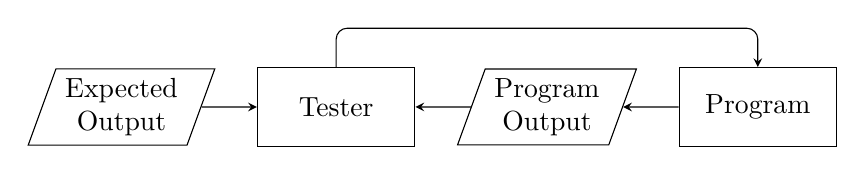
\begin{tikzpicture}
		\node (Tester)[process]{Tester};
		\node (Program Output)[io, right = 2em of Tester, align=center]{Program\\Output};
		\node (Program)[process, right = 2em of Program Output]{Program};
		\node (Expected Output)[io, left = 2em of Tester, align=center]{Expected\\Output};
		\draw [-stealth] (Expected Output) -- (Tester);
		\draw [-stealth] (Program Output) -- (Tester);
		\draw [-stealth] (Program) -- (Program Output);
		\draw [-stealth, rounded corners] (Tester.north) -- (0,1) -| (Program.north);
	\end{tikzpicture}
	\caption{External Program Side-effect Comparison Overview}
	\label{fig:autofigure1}
\end{figure}


\subsection{Internal Program Unit Testing}

Unit testing is assumed to be the evaluation of individual discrete code components within a tested program by comparing internal program state such as a function return value to a known expected state that has been pre-generated by a sample solution.

In internal program unit testing, the execution and collection of results from internal unit test cases can be used to determine whether expected behaviour has been achieved.

As a benefit, testing internal code components permits for finer control on the determination of program correctness by exposing internal functions instead of being reliant on observing side-effects. However, this benefit is traded off with the difficulty of unit testing more complex programs which may not be able the share the same unit testing framework throughout all components.

The interactions between the code tester and test program can be summarised in \autoref{fig:autofigure2}.

\begin{figure}[h]
	\centering
	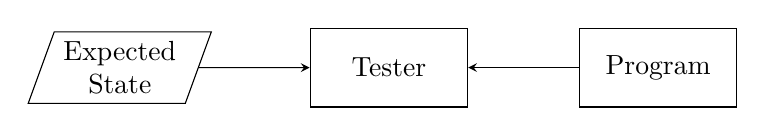
\begin{tikzpicture}
		\node (Tester)[process]{Tester};
		\node (Program)[process, right = 4em of Tester]{Program};
		\node (Expected Output)[io, left = 4em of Tester, align=center]{Expected\\State};
		\draw [-stealth] (Expected Output) -- (Tester);
		\draw [-stealth] (Program) -- (Tester);
	\end{tikzpicture}
	\caption{Internal Program Unit Testing Overview}
	\label{fig:autofigure2}
\end{figure}

\subsection{Differences}
It is possible to argue that both \textit{side-effect comparison} and \textit{unit testing} seem very similar since each technique checks program ``state" after executing some code. However, this thesis was unable to find any other suitable and usable technique in determining program correctness within a reasonable amount of time. For example, formal methods would be difficult to implement in a general way while artificial intelligence would be too unpredictable for the purposes of this thesis.

\clearpage
\section{Software Containerisation}
Containerisation is generally accepted as the ``packaging together of code with all its necessary components [such that packages] are isolated in their own container". This allows containers to be run consistently in any environment and on any infrastructure regardless of the operating system. More importantly, containers are isolated from the rest of a host system which will be an important feature for this thesis \cite{containerisationGeneral}.
In order to understand how containerisation works and how it could be of benefit to this thesis, we need to understand how \textit{Linux namespaces} work to provide containerisation.

\subsection{Linux Namespaces}
Namespaces are a Linux kernel feature introduced in 2002 which permits the isolation of a process from the rest of the host system. To provide finer control over the individual aspects of a process, there are currently eight namespaces that can be created as shown in \autoref{tab:table2}. This provides the ability to isolate a process without removing aspects such as network access which a user may wish to keep intact. All of these namespaces with the exception of the user namespace (Linux >= 3.8) require the \textit{CAP\_SYS\_ADMIN} kernel capability to be enabled. No privilege is required for the user namespace with Linux 3.8 or above \cite{containerisationManPage}.

\begin{table}[h]
	\centering
	\begin{tabular}{ll}
		\toprule
		\textbf{Namespace} & \textbf{Resources Isolated} \\
		\midrule
		Cgroup & Cgroup root directory (system resource allocations such as cpu or memory) \\
		IPC & System V IPC, POSIX message queues \\
		Network & Network devices, stacks, ports, etc. \\
		Mount  & Mount points (file system mounts) \\
		PID & Process IDs (Process ID table) \\
		Time & Boot and monotonic clocks \\
		User & User and group IDs (ability for a process to have root privilege within the namespace) \\
		UTS & Hostname and NIS domain name \\
		\bottomrule
	\end{tabular}
	\caption{Linux namespaces and resources isolated by each namespace}
	\label{tab:table2}
\end{table}

Isolating all eight namespaces allows a process to be mostly separate from the host system which can serve as the base for a container instance. Most widely used container engines such as \textit{Docker} and \textit{Podman} rely upon namespaces among other techniques such as overlay filesystems to provide containerisation \cite{dockerUnderlying}\cite{podmanUnderlying}.

\subsection{Rootless Containers}
The majority of popular container engines require the host system to execute the engine with root privileges in order to deliver full functionality. In recent years, the idea of \textit{rootless containers} has gained traction to counter the possible damage to a host system if a container run under root privileges is escaped by a malicious program which would then also assume root permissions. Although good practices by the user can minimise the risk of a container escape, undiscovered vulnerabilities and user error can bypass the efforts taken by the user. \textit{Rootless containers} mostly remove the risk as any malicious programs escaping a container will no longer assume privileged access automatically.

As a result of the benefits, industry standard container engines such as \textit{Docker} and \textit{Podman} have introduced rootless versions of their engines but are severely lacking in task-specific documentation such as usage or troubleshooting due to the relatively poor uptake by a majority of users \cite{rootlessDocker}. These users usually do not know that a rootless mode exists, require features that are only available with privileged execution or have simply accepted or ignored the risk.

With this overview, this thesis will refer to ``containerisation" as one of its main benefits which is the isolation of an executing program from the remainder of a host system. The other main benefits such as software portability are noted but did not have a functional role in this thesis outside of potential future work.

\unchapter{3}{Related Works}

It is important to explore some existing work which could influence the design towards a chosen direction. In particular, this thesis explores and evaluates the following related works:
\begin{itemize}
	\item \textit{autotest} - the current automated code testing tool used for introductory programming courses at UNSW \cite{Autotest}.
	\item \textit{check50} - another implementation of an automated code testing tool used in the CS50 introductory programming course at Harvard University \cite{check50}.
	\item \textit{gtest} - a C++ unit testing framework used by Google and the programming community \cite{gtest}.
\end{itemize}
Historic and minimally relevant implementations are also mentioned for completeness.

\section{autotest}

As mentioned in Chapter 1, \textit{autotest} is a software package designed by Andrew Taylor to fulfil the purpose of an automatic code testing tool and has become the standard code testing tool for introductory programming courses at UNSW.

\subsection{Implementation \& Usage Overview}

\textit{autotest} is a tool that primarily follows the \textit{external program side-effect comparison} methodology to automatically determine the correctness of a tested program which can be seen in \autoref{fig:autotest1}. \textit{autotest} is written in Python but does expose some Bash shell and Perl script interfaces as a result of its historical relation with the earlier script by Mei Cheng Whale.

\begin{figure}[h]
	\centering
	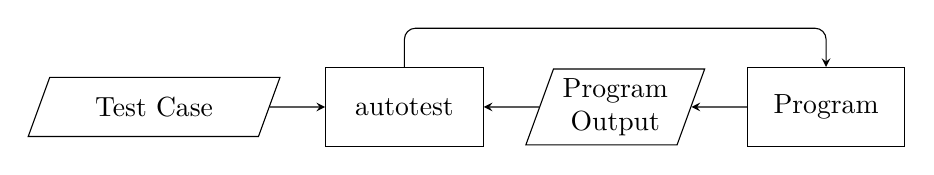
\begin{tikzpicture}
		\node (Tester)[process]{autotest};
		\node (Program Output)[io, right = 2em of Tester, align=center]{Program\\Output};
		\node (Program)[process, right = 2em of Program Output]{Program};
		\node (Expected Output)[io, left = 2em of Tester, align=center]{Test Case};
		\draw [-stealth] (Expected Output) -- (Tester);
		\draw [-stealth] (Program Output) -- (Tester);
		\draw [-stealth] (Program) -- (Program Output);
		\draw [-stealth, rounded corners] (Tester.north) -- (0,1) -| (Program.north);
	\end{tikzpicture}
	\caption{autotest High-level Architecture}
	\label{fig:autotest1}
\end{figure}

In terms of usage, \textit{autotest} provides a simplified interface to define multiple test cases with custom test parameters and environment in accordance with the needs of the user. In particular, the ability to set a time limit for each test case is valuable in handling cases where code may have an unintentional infinite loop, a common mistake made by beginners to programming.

\begin{figure}[h]
	\centering
	\begin{lstlisting}[linewidth=\linewidth]
files=is_prime.c
		
1 stdin="39" expected_stdout="39 is not prime\n"
2 stdin="42" expected_stdout="42 is not prime\n"
3 stdin="47" expected_stdout="47 is prime\n"
	\end{lstlisting}
	\caption{autotest Example Test Cases}
	\label{fig:autotest2}
\end{figure}

Files containing these test case specifications (\autoref{fig:autotest2}) can be saved to a directory and easily utilised by a wrapper script (\autoref{fig:autotest3}) which generalises and simplifies execution of the tool via abstraction of certain details from the intended end-user:

\begin{figure}[h]
	\centering
	\begin{lstlisting}[language=bash, breaklines=true, linewidth=\linewidth]
#!/bin/sh

parameters="
default_compilers = {'c' : [['gcc', '-Werror', '-std=gnu11', '-g', '-lm']]}
"

exec <path_to_autotest>/autotest.py -a <path_to_test_dir> --parameters "$parameters" "$@"
	\end{lstlisting}
	\caption{autotest Wrapper Script}
	\label{fig:autotest3}
\end{figure}

Upon execution of \textit{autotest} with a correct \textit{is\_prime.c}, the output shown in \autoref{fig:autotest4} is expected which informs the user that the provided test cases have passed. In this particular case, the tested program has successfully provided the expected output as defined by each of the test cases.

\begin{figure}[h]
	\centering
	\begin{lstlisting}[breaklines=true, linewidth=\linewidth]
gcc -Werror -std=gnu11 -g -lm -o is_prime is_prime.c
Test 1 (is_prime) - passed
Test 2 (is_prime) - passed
Test 3 (is_prime) - passed
3 tests passed 0 tests failed
	\end{lstlisting}
	\caption{autotest execution on correct program}
	\label{fig:autotest4}
\end{figure}

In the event that \textit{autotest} is executed with a flawed \textit{is\_prime.c}, \textit{autotest} will report to the user on the cause of the failure of a test case whether it is a mismatch in side-effects in the case of \autoref{fig:autotest5} or other cause such as compilation failure. Over the lifetime of \textit{autotest}, the unique situations that the tool can detect has increased which in turn provides users with additional targeted information and context.

This information is useful to both student and staff as it may be difficult to manually analyse the differences in larger amounts of side-effects created from more complex programs or program executions.  As such, it is one of the defining features that separates \textit{autotest} from other implementations.

\begin{figure}[h]
	\centering
	\begin{lstlisting}[breaklines=true, linewidth=\linewidth]
gcc -Werror -std=gnu11 -g -lm -o is_prime is_prime.c
Test 1 (is_prime) - passed
Test 2 (is_prime) - passed
Test 3 (is_prime) - failed (Incorrect output)
Your program produced this line of output:
47 is not prime

The correct 1 lines of output for this test were:
47 is prime

The difference between your output(-) and the correct output(+) is:
- 47 is not prime
?      ----

+ 47 is prime

The input for this test was:
47
You can reproduce this test by executing these commands:
gcc -Werror -std=gnu11 -g -lm -o is_prime is_prime.c
echo -n 47 | is_prime
2 tests passed 1 tests failed
	\end{lstlisting}
	\caption{autotest execution on incorrect program}
	\label{fig:autotest5}
\end{figure}

It is noted that to ensure a test program's full compliance to a given specification with \textit{autotest}, sufficient test cases to cover all edge cases and standard execution will be required. This can be a challenge depending on the complexity of the specification but it is noted that testing coverage is out of scope for \textit{autotest}.

\subsection{Benefits}

Further analysis of \textit{autotest} and its usage at UNSW can provide the following list of benefits for this thesis as an inspiration:
\begin{itemize}
	\item \textbf{\textit{autotest} has been proven to be mostly reliable at UNSW} - There have been undocumented reports of rare autotest crashes when being run in a distributed fashion but no documented reports could be found of the issue affecting administration of coding assessments within UNSW \cite{AutotestConversation}.
	\item \textbf{\textit{autotest} is able to support any programming language in which \textit{autotest} can detect and compare side-effects to determine program correctness} - This assists greatly in the usability of \textit{autotest} by courses that do not share an identical programming language as \textit{external program side-effect comparison} is a language-agnostic methodology.
	\item \textbf{\textit{autotest} exposes many parameters in the test case specification which allows users to have finer control over the test execution environment} - Some specifications that \textit{autotest} may want to test could require specialised testing environments for its test cases.
	\item \textbf{\textit{autotest} has a side-effect comparison module that provides meaningful information on differences between actual and expected output in the event of a test failure} - This is one of the most defining components of \textit{autotest} in the assistance it provides to users.
\end{itemize} 

\subsection{Limitations}\label{autotestLimitations}

Despite the benefits of \textit{autotest}, there are unfortunately some limitations that make \textit{autotest} unsuitable for continued use and have motivated this thesis:
\begin{itemize}
	\item \textbf{\textit{autotest} was not designed for long term maintainability and feature extensibility} - This is evident in the difficulty to change major components of \textit{autotest} without significant and difficult overhaul on large amounts of the code base as seen in the 2021 improvements by UNSW CSE.
	\item \textbf{\textit{autotest} has incorrect, outdated and insufficient documentation} - Although the mistakes in documentation are relatively minor such as typos, the insufficient and outdated information has been difficult to rectify. This has hindered the ability of contributors to understand how \textit{autotest} works at a deeper level and obstructed first-time users from utilising \textit{autotest} to its fullest ability.
	\item \textbf{\textit{autotest} was not designed for security which is of concern in modern times} - When code testing foreign code as a result of marking, the current iteration of \textit{autotest} has no in-built protections against potentially malicious code such as deletion of system files (eg. ``\textit{sudo rm -rf /}"). This can be alleviated via external means such as limiting permissions for the user executing \textit{autotest} but this is only a short term solution.
	\item \textbf{\textit{autotest} has performance issues as a result of its original design} - \textit{autotest} was not originally intended to be utilised at the scale as it is today. As such, its most significant performance issue is the single-threaded nature of \textit{autotest} where there is no accepted implementation to execute unrelated tests in parallel \cite{AutotestParallelisation}.
\end{itemize}

\clearpage
\section{check50}

\textit{check50} is a software package designed by Chad Sharp and others at Harvard University to fulfil the purpose of an automatic code testing tool. Similar to \textit{auotest}, \textit{check50} which was first introduced in 2012 has also become the standard code testing tool for the \textit{CS50: Introduction to Computer Science} course at Harvard University.

\subsection{Implementation \& Usage Overview}

\textit{check50} is a tool that primarily follows the \textit{external program side-effect comparison} to automatically determine the correctness of a tested program which can be seen in \autoref{fig:check501}. \textit{check50} is written in Python and receives active maintenance and development efforts via a private repository \cite{check50Github}.

\begin{figure}[h]
	\centering
	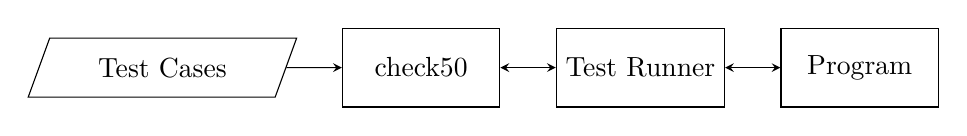
\begin{tikzpicture}
		\node (Tester)[process]{check50};
		\node (Tests)[io, left = 2em of Tester, align=center]{Test Cases};
		\node (Test Runner)[process, right = 2em of Tester]{Test Runner};
		\node (Program)[process, right = 2em of Test Runner]{Program};
		\draw [-stealth] (Tests) -- (Tester);
		\draw [stealth-stealth] (Tester) -- (Test Runner);
		\draw [stealth-stealth] (Test Runner) -- (Program);
	\end{tikzpicture}
	\caption{check50 High-level Architecture}
	\label{fig:check501}
\end{figure}

In terms of usage, \textit{check50} provides a simple framework for defining the test cases as well as an easy-to-use API that abstracts common tasks such as compiling and running away from the user. In line with the goals of \textit{check50}, the creation of test cases known as ``checks" is simplified into a chain of functions in Python similar to that seen in functional languages such as Haskell. YAML checks can also be defined but are converted into Python automatically on execution of these checks by \textit{check50}.

\begin{figure}[h]
	\centering
	\begin{lstlisting}[language=python, breaklines=true, linewidth=\linewidth, tabsize=4]
import check50
import check50.c

@check50.check()
def exists():
	"""hello.c exists"""
	check50.exists("hello.c")

@check50.check(exists)
def compiles():
	"""hello.c compiles"""
	check50.c.compile("hello.c", lcs50=True)

@check50.check(compiles)
def emma():
	"""responds to name Emma"""
	check50.run("./hello").stdin("Emma").stdout("Emma").exit()
	\end{lstlisting}
	\caption{check50 Example Test Cases (Checks)}
	\label{fig:check502}
\end{figure}

Files containing these checks (\autoref{fig:check502}) can be saved to a directory locally or online to be executed as a ``slug" which is the relative path to the directory containing checks. Since \textit{check50} is officially recommended to be installed as a pip package, execution of \textit{check50} on a slug is relatively simple as seen in \autoref{fig:check503} \cite{check50Docs}. It is also observed that upon execution of \textit{check50} with a correct \textit{hello.c}, the tool reports to the user that the provided checks have passed. In this particular case, the tested program has successfully completed all checks as defined.

\begin{figure}[h]
	\centering
	\begin{lstlisting}[breaklines=true, linewidth=\linewidth]
$ check50 <path_to_example_checks>
:) hello.c exists
:) hello.c compiles
:) responds to name Emma
	\end{lstlisting}
	\caption{check50 execution on correct program}
	\label{fig:check503}
\end{figure}

In the event \textit{check50} is executed with a flawed \textit{hello.c}, \textit{check50} will report to the user on the failure of a test case whether it is a mismatch in side-effects in the case of \autoref{fig:check504} or other cause such as compilation failure. \textit{check50} supports the provision of a hint string in the failure of the test case but this must be manually set by the test writer and may potentially distract from the issue if the hint is not appropriate.

\begin{figure}[h]
	\centering
	\begin{lstlisting}[breaklines=true, linewidth=\linewidth]
$ check50 <path_to_example_checks>
:) hello.c exists
:) hello.c compiles
:( responds to name Emma
	expected "Emma\n", not "emma\n"
	<hint_string_here>
	\end{lstlisting}
	\caption{check50 execution on incorrect program}
	\label{fig:check504}
\end{figure}

Similarly to \textit{autotest}, to ensure a test program's full compliance to a given specification with \textit{check50}, sufficient checks to cover all edge cases and standard execution will be required which can be a challenge depending on the complexity of the specification. However, evaluation of checks for a specification is out of scope for \textit{check50}. 

\subsection{Benefits}

Further analysis of \textit{check50} can provide the following list of benefits for this thesis as an inspiration:
\begin{itemize}
	\item \textbf{\textit{check50} test cases or checks are very easy to create} - There are many examples of checks that are available publicly and the difficulty of creating checks for basic programs is significantly lower than \textit{autotest} \cite{check50Examples}.
	\item \textbf{\textit{check50} is theoretically able to support any programming language} - This assists greatly in the usability of \textit{check50} by courses that do not share an identical programming language as \textit{check50} is declared to be theoretically language-agnostic assuming the user implements the necessary tooling for the language such as the framework and API.
	\item \textbf{\textit{check50} maintains extensive and up-to-date documentation} - This is a significant benefit as the extensive documentation supports users in their understanding on the more confusing components of \textit{check50} which has made usage of the tool and code contributions much easier.
	\item \textbf{\textit{check50} has a module that converts \textit{check50} output into a HTML page that improves readability of results for users who may find terminal output difficult to read} - This is one of the most defining components of \textit{check50} in the benefit of this thesis as it improves accessibility of the tool to students who may have difficulties with sight.
	\item \textbf{\textit{check50} implements containerisation of checks as a security measure against potentially malicious code and can be configured to run both remotely or locally} - This is an important feature that offers significant long term advantages such as infrastructure safety and scalability by keeping infrastructure secure and permitting users to run checks locally respectively. As such, it is a significant advantage that \textit{check50} has over \textit{autotest}.
	\item \textbf{\textit{check50} supports concurrent execution of tests} - Concurrent execution of unrelated tests takes advantage of the full resources offered by a computer to evaluate all checks in a minimal amount of time which increases performance and efficiency. As an added benefit, \textit{check50} checks have the ability to define an execution order or dependency graph which ensures that certain checks such as tests on the existence of certain files and compilation are executed first before checks that depend on them. 
\end{itemize} 

\subsection{Limitations}

Despite the benefits of \textit{check50}, there are unfortunately some limitations that make \textit{check50} nonviable for immediate use and have motivated this thesis:

Assume \textit{harnessing} to be programs and tooling that is specifically created for the purposes of creating side-effects or other usable information from programs that do not generate such information alone. An example of \textit{harnessing} would be a test program that outputs the return value of a function that is not exposed to the user under normal operating conditions. 

\begin{itemize}
	\item \textbf{\textit{check50} has an emphasis on the easy creation of tests which has resulted in larger amounts of abstractions and complicated the execution of complex programs} - This could be mitigated by harnessing the complex programs to work with \textit{check50} but this is a short term solution and could involve significant work by the user to implement.
	\item \textbf{\textit{check50} has no official support for languages outside of C, Python and Python Flask} - Although support can be implemented for different languages, there is likely a non-trivial amount of work that is necessary with no guarantee that the implementation by the user will be correct. This could once again be mitigated by harnessing but the same flaw of being a short term solution and potentially requiring significant work remains.
\end{itemize}

\clearpage
\section{gtest}

\textit{gtest} is a testing and mocking framework originally designed by Google to fulfil the purpose of testing Google's internal C++ projects. \textit{gtest} has since been released to the public in 2008 and has become one of the most popular C++ testing tools that is publicly available as open source software.

\subsection{Implementation \& Usage Overview}

\textit{gtest} is a tool that primarily follows the \textit{internal program unit testing} methodology to automatically determine the correctness of a tested program which can be seen in \autoref{fig:gtest1}. It could theoretically support \textit{external program side-effect comparison} but it would require significant harnessing efforts that may not carry over for different specifications. \textit{gtest} is written in C++ and receives active maintenance and development efforts by both Google and the open source software community.

\begin{figure}[h]
	\centering
	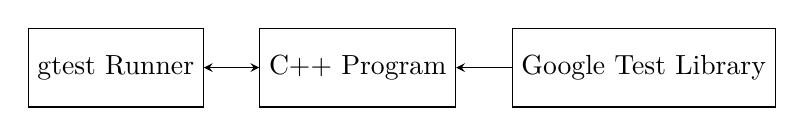
\begin{tikzpicture}
		\node (Tester)[process]{gtest Runner};
		\node (Program)[process, right = 2em of Tester]{C++ Program};
		\node (Tooling)[process, right = 2em of Program]{Google Test Library};
		\draw [stealth-stealth] (Tester) -- (Program);
		\draw [-stealth] (Tooling) -- (Program);
	\end{tikzpicture}
	\caption{gtest High-level Architecture}
	\label{fig:gtest1}
\end{figure}

In terms of usage, \textit{gtest} approaches defining of test cases in a unique way in comparison to \textit{autotest} or \textit{check50}. In particular, test cases are able to specifically target internal components of a tested program such as functions without harnessing unlike \textit{autotest} and \textit{check50} that can only target the tested program as a whole without the use of harnessing.

\begin{figure}[h]
	\centering
	\begin{lstlisting}[language=c++, breaklines=true, linewidth=\linewidth]
// test.h
#include "is_prime.h"
#include <gtest/gtest.h>

TEST(IsPrimeTest, Positive) {
	EXPECT_FALSE(IsPrime(4));
	EXPECT_TRUE(IsPrime(5));
	EXPECT_FALSE(IsPrime(6));
	EXPECT_TRUE(IsPrime(23));
}
	\end{lstlisting}
	\caption{gtest Example Test Cases}
	\label{fig:gtest2}
\end{figure}

Files containing these test case specifications (\autoref{fig:gtest2}) can be saved to a directory and executed via a \textit{gtest} runner which will automatically collect all tests from linked files when compiled and run (\autoref{fig:gtest3}):

\begin{figure}[h]
	\centering
	\begin{lstlisting}[language=c++, breaklines=true, linewidth=\linewidth]
// main_test.cc
#include <gtest/gtest.h>

#include "test.h"
// link all other test specification files here

int main(int argc, char **argv) {
	testing::InitGoogleTest(&argc, argv);
	return RUN_ALL_TESTS();
}
	\end{lstlisting}
	\caption{gtest runner Source Code}
	\label{fig:gtest3}
\end{figure}

\begin{figure}[h]
	\centering
	\begin{lstlisting}[breaklines=true, linewidth=\linewidth]
$ ./main_test
[==========] Running 1 test from 1 test suite.
[----------] Global test environment set-up.
[----------] 1 test from IsPrimeTest
[ RUN      ] IsPrimeTest.Positive
[       OK ] IsPrimeTest.Positive (0 ms)
[----------] 1 test from IsPrimeTest (0 ms total)

[----------] Global test environment tear-down
[==========] 1 test from 1 test suite ran. (0 ms total)
[  PASSED  ] 1 test.
	\end{lstlisting}
	\caption{gtest runner execution on correct program}
	\label{fig:gtest4}
\end{figure}

\begin{figure}[h]
	\centering
	\begin{lstlisting}[breaklines=true, linewidth=\linewidth]
$ ./main_test
[==========] Running 1 test from 1 test suite.
[----------] Global test environment set-up.
[----------] 1 test from IsPrimeTest
[ RUN      ] IsPrimeTest.Positive
main_test.cc:17: Failure
Value of: IsPrime(23)
Actual: false
Expected: true
[  FAILED  ] IsPrimeTest.Positive (0 ms)
[----------] 1 test from IsPrimeTest (0 ms total)

[----------] Global test environment tear-down
[==========] 1 test from 1 test suite ran. (0 ms total)
[  PASSED  ] 0 tests.
[  FAILED  ] 1 test, listed below:
[  FAILED  ] IsPrimeTest.Positive

1 FAILED TEST
	\end{lstlisting}
	\caption{gtest runner execution on incorrect program}
	\label{fig:gtest5}
\end{figure}

Upon execution of the \textit{gtest runner} with a correct \textit{is\_prime.cc} and \textit{is\_prime.h}, the output shown in \autoref{fig:gtest4} is expected which informs the user that the provided test cases have passed. In this particular case, all assertions of the \textit{isPrimeTest} test case have passed.

In the event \textit{gtest runner} is executed with a flawed \textit{is\_prime.cc} or \textit{is\_prime.h}, \textit{gtest} will report to the user on the cause of the failure of a test case such as a deviation from expected behaviour as seen in \autoref{fig:gtest5}.

To ensure a test program's full compliance to a given specification with \textit{gtest}, sufficient test cases to cover all edge cases and standard execution will be required which can be a challenge depending on the complexity of the specification. However, checks on the creation of tests is out of scope for \textit{gtest}.

\subsection{Benefits}

Further analysis of \textit{gtest} can provide the following list of benefits for this thesis as an inspiration:
\begin{itemize}
	\item \textbf{\textit{gtest} maintains extensive and up-to-date documentation with a large community of users} - This is a significant benefit as \textit{gtest} as a whole can be perceived as complicated and confusing but many community made tutorials and guides exist on the internet to solve most issues.
	\item \textbf{\textit{gtest} supports concurrent execution of tests} - Concurrent execution of unrelated tests takes advantage of the full resources offered by a computer to evaluate all test cases in a minimal amount of time which increases performance and efficiency. However, \textit{gtest} offers no methods to guarantee that tests will be executed in a certain order unlike \textit{check50}. 
\end{itemize} 

\subsection{Limitations}

Despite the benefits of \textit{gtest}, there are unfortunately some limitations that make \textit{gtest} unsuitable for use:
\begin{itemize}
	\item \textbf{\textit{gtest} is not designed to test whole programs and can have trouble detecting side-effects such as the existence of files without significant harnessing} - This is expected for software that implements \textit{internal program unit testing} as a methodology but still remains a significant limitation of \textit{gtest} for use as an automated code testing tool.
	\item \textbf{\textit{gtest} does not sufficiently support test execution environment configuration easily} - \textit{Internal program unit testing} frameworks are not expected to manage an external test environment but the difficulty and lack of configuration within \textit{gtest} could prevent the testing of programs that may rely on a specialised environment.
	\item \textbf{\textit{gtest} is generally difficult to use as an automated code testing tool} - \textit{gtest} is difficult to configure and utilise for most users and far better tools such as \textit{autotest} and \textit{check50} exist for a baseline design.
\end{itemize}

\section{Other \& Historic Works}
See these other and historic works that have had minimal but relevant impact on this thesis as an exploration on the progression of each aforementioned automated code testing methodology throughout history: \textbf{JUnit} (Internal Program Unit Testing) \cite{junit}, \textbf{BAGS} (Primitive External Program Side-effect Comparison) \cite{bags}, \textbf{Kassandra} (External Program Side-effect Comparison) \cite{kassandra} and \textbf{TRY} (External Program Side-effect Comparison) \cite{try}. 

\unchapter{4}{Approach}

\section{Requirements}

The initial problem statement of introducing a replacement automated code testing tool is quite broad, and the required design will depend highly on the chosen automated testing approach. In particular, it would be impossible to have one solution that will immediately satisfy the demands of all users.

Therefore it is important to lay out the desired requirements and design goals for an ideal solution before choosing a proposed approach for the implementation.

\subsection{Design Goals}

In accordance with the thesis aim, the design goals for the project will emphasise the following properties:

\begin{itemize}
	\item \textbf{Accessibility} - The design should allow new users to easily integrate this automated code testing tool into their coding assessments.
	\item \textbf{Familiarity} - Existing users of \textit{autotest} should not observe the proposed solution and its usage to be completely independent of the former.
	\item \textbf{Performance \& Efficiency} - The proposed implementation should be observed to have comparable if not better performance than the existing \textit{autotest}. Benchmarking of \textit{autotest} and the proposed implementation will be performed to verify this goal.
	\item \textbf{Maintainability} - The design should be adequately documented, support an ease of maintainability and possible extension of features via the appropriate architectural decisions.
	\item \textbf{Security} - The design should implement or consider the addition of security as it has been a concern for various implementations of an \textit{automated code testing tool} in the protection of user hardware against potentially malicious code.
\end{itemize}

It is noted that most of these goals are qualitative and can not be quantitatively measured outside of reader observation. The thesis will attempt to quantify these goals within the properties of each proposed design approach but it will still be dependent on the reader's interpretation.

\clearpage
\section{Design}

From the evaluation of the related works, this thesis evaluates two potential design approaches to the solution that fulfils the design goals outlined above, one of these two approaches is then chosen for the project. Implementation details for each design approach are important but defining a ``target" architecture design is considered to be of greater importance as it cannot be easily changed once development begins.

\subsection{check50 Approach}\label{check50Approach}

In this approach, the architectural design will be similar to that of \textit{check50} as shown in \autoref{fig:approach1-1} including the design for definition of test cases and as such, the methodology to determine correctness of a tested program will be \textit{external program side-effect comparison}.

\begin{figure}[h]
	\centering
	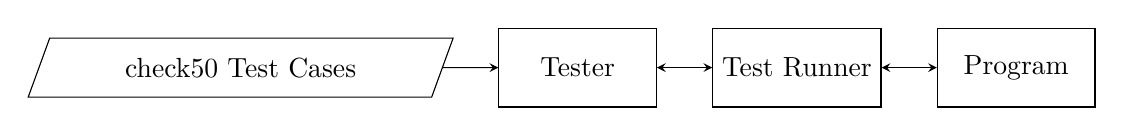
\begin{tikzpicture}
		\node (Tester)[process]{Tester};
		\node (Tests)[io, left = 2em of Tester, align=center]{check50 Test Cases};
		\node (Test Runner)[process, right = 2em of Tester]{Test Runner};
		\node (Program)[process, right = 2em of Test Runner]{Program};
		\draw [-stealth] (Tests) -- (Tester);
		\draw [stealth-stealth] (Tester) -- (Test Runner);
		\draw [stealth-stealth] (Test Runner) -- (Program);
	\end{tikzpicture}
	\caption{check50 Approach - High-level Architecture}
	\label{fig:approach1-1}
\end{figure}

This approach allows the project to utilise \textit{check50} as a ``baseline" for both performance and correctness testing of the solution which will aid in the development process by being a reference solution that can be compared with.

To further develop the approach, a solution implementing this approach would work like so (at a high level):
\begin{enumerate}
	\item The \textit{Tester} will read in the appropriate \textit{test cases} and any other relevant information to parse into individual test cases with the relevant parameters set (timeout period, test input, expected output etc).
	\item The \textit{Tester} will ``spin up"/initialise a configured amount of \textit{Test Runner} processes which will each individually consume a test case for independent execution.
	\item When the \textit{Test Runner} completes execution of a test which may involve an external \textit{Program}, the \textit{Test Runner} will return its result back to the \textit{Tester} and consume another test for execution if one exists. If no more tests exist, the waiting \textit{Test Runner} will ``spin down"/shut down.
	\item Throughout steps 2 and 3, the \textit{Tester} will report to the user on test execution progress but once all tests results have been gathered, a report will be generated for the user on test successes and failures.
\end{enumerate}

\subsection{autotest Approach}

In this approach, the architecture is similar to the \textit{check50 approach} in \autoref{check50Approach} but with the distinct change that the design of the test case definitions will be that of the existing \textit{autotest}.

\begin{figure}[h]
	\centering
	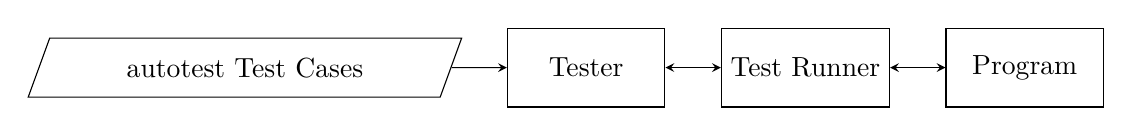
\begin{tikzpicture}
		\node (Tester)[process]{Tester};
		\node (Tests)[io, left = 2em of Tester, align=center]{autotest Test Cases};
		\node (Test Runner)[process, right = 2em of Tester]{Test Runner};
		\node (Program)[process, right = 2em of Test Runner]{Program};
		\draw [-stealth] (Tests) -- (Tester);
		\draw [stealth-stealth] (Tester) -- (Test Runner);
		\draw [stealth-stealth] (Test Runner) -- (Program);
	\end{tikzpicture}
	\caption{autotest Approach - High-level Architecture}
	\label{fig:approach2-1}
\end{figure}

The original architecture of \textit{autotest} has been abandoned in this approach as the \textit{check50} architecture is more suitable to the aforementioned design goals.

Thus, the solution implementing this approach will be identical to the \textit{check50 approach} and has been omitted as it is available in \autoref{check50Approach}.

\subsection{Chosen Approach}

Evaluation of each approach was made by considering fulfilment of the design goals aforementioned above. \autoref{tab:table3} lists if each approach satisfies each design requirement.

\begin{table}[h]
	\centering
	\begin{tabular}{lll}
		\toprule
		\textbf{Requirement} & \textbf{check50 Approach} & \textbf{autotest Approach} \\
		\midrule
		Accessibility    & Yes (by design) & Yes (by design) \\
		Familiarity      & No  & Yes \\
		Performance \& Efficiency & Unknown & Unknown \\
		Maintainability  & Yes (Technical Debt Management) & Yes (Technical Debt Management) \\
		Security 		 & Planned & Planned \\
		\bottomrule
	\end{tabular}
	\caption{Evaluation of the check50 and autotest approach against the stated requirements}
	\label{tab:table3}
\end{table}

As seen from \autoref{tab:table3}, neither approach completely matches the requirements laid out, however the \textit{autotest approach} is close and will serve as an appropriate start for the project over the alternative.

It is noted that some components of the test case definition design and backend design of \textit{check50} could be considered to be superior to that of \textit{autotest}. As these features are implementations details and are not greatly affected in respect to the chosen architecture, decisions on whether these features will be included in the solution were deferred until implementation. In general, the decisions were assessed upon fulfilling the design goals as much as possible.

\unchapter{5}{Implementation}
To prevent confusion between the design of the new solution and the existing \textit{autotest}, this thesis will refer to the new automated code testing tool as \textbf{\textit{lemontest}} which also serves as its interim name.
Due to time constraints and unforeseen roadblocks, it was only possible to achieve the thesis aims by redesigning and implementing the majority of \textit{autotest} functionality.
As per the design goals, \textit{autotest} served as a ``baseline" for which \textit{lemontest} would be built and improve upon. However, \textit{lemontest} can still be considered a ``bottom-up" implementation of an automated code testing tool as evident by the following:
\begin{enumerate}
	\item Architecture of \textit{autotest} is discarded for a modular design which serves as a base to fulfil the design goals and approach chosen for \textit{lemontest}.
	\item Each module is given a clear, ideally single responsibility (high cohesion) and is designed to limit inter-dependency with other modules (low coupling).
	\item Modern programming techniques and good practices such as containerisation and code documentation respectively are implemented with the relevant modules to deliver on the stipulations of the design goals.
	\item Feature parity with \textit{autotest} is achieved whilst maintaining the design goals.
\end{enumerate}

\section{Architecture}\label{architecture}
Recall from the related works section (\autoref{autotestLimitations}) that whilst the original \textit{autotest} delivered on its purpose as an automated marking tool, it is plagued with a lack of clear structure in its design. Although \textit{autotest} was never intended to be expanded to the extent it is today, the lack of a clear architecture has made it significantly difficult to extend \textit{autotest} with new functionality. \textit{Lemontest} improves on this limitation by embracing a modular architecture which isolates the discrete pieces of functionality seen in \textit{autotest} into individual modules with little to no dependencies with each other as shown in \autoref{fig:architecture}.

\begin{figure}[h]
	\centering
	\makebox[\textwidth][c]{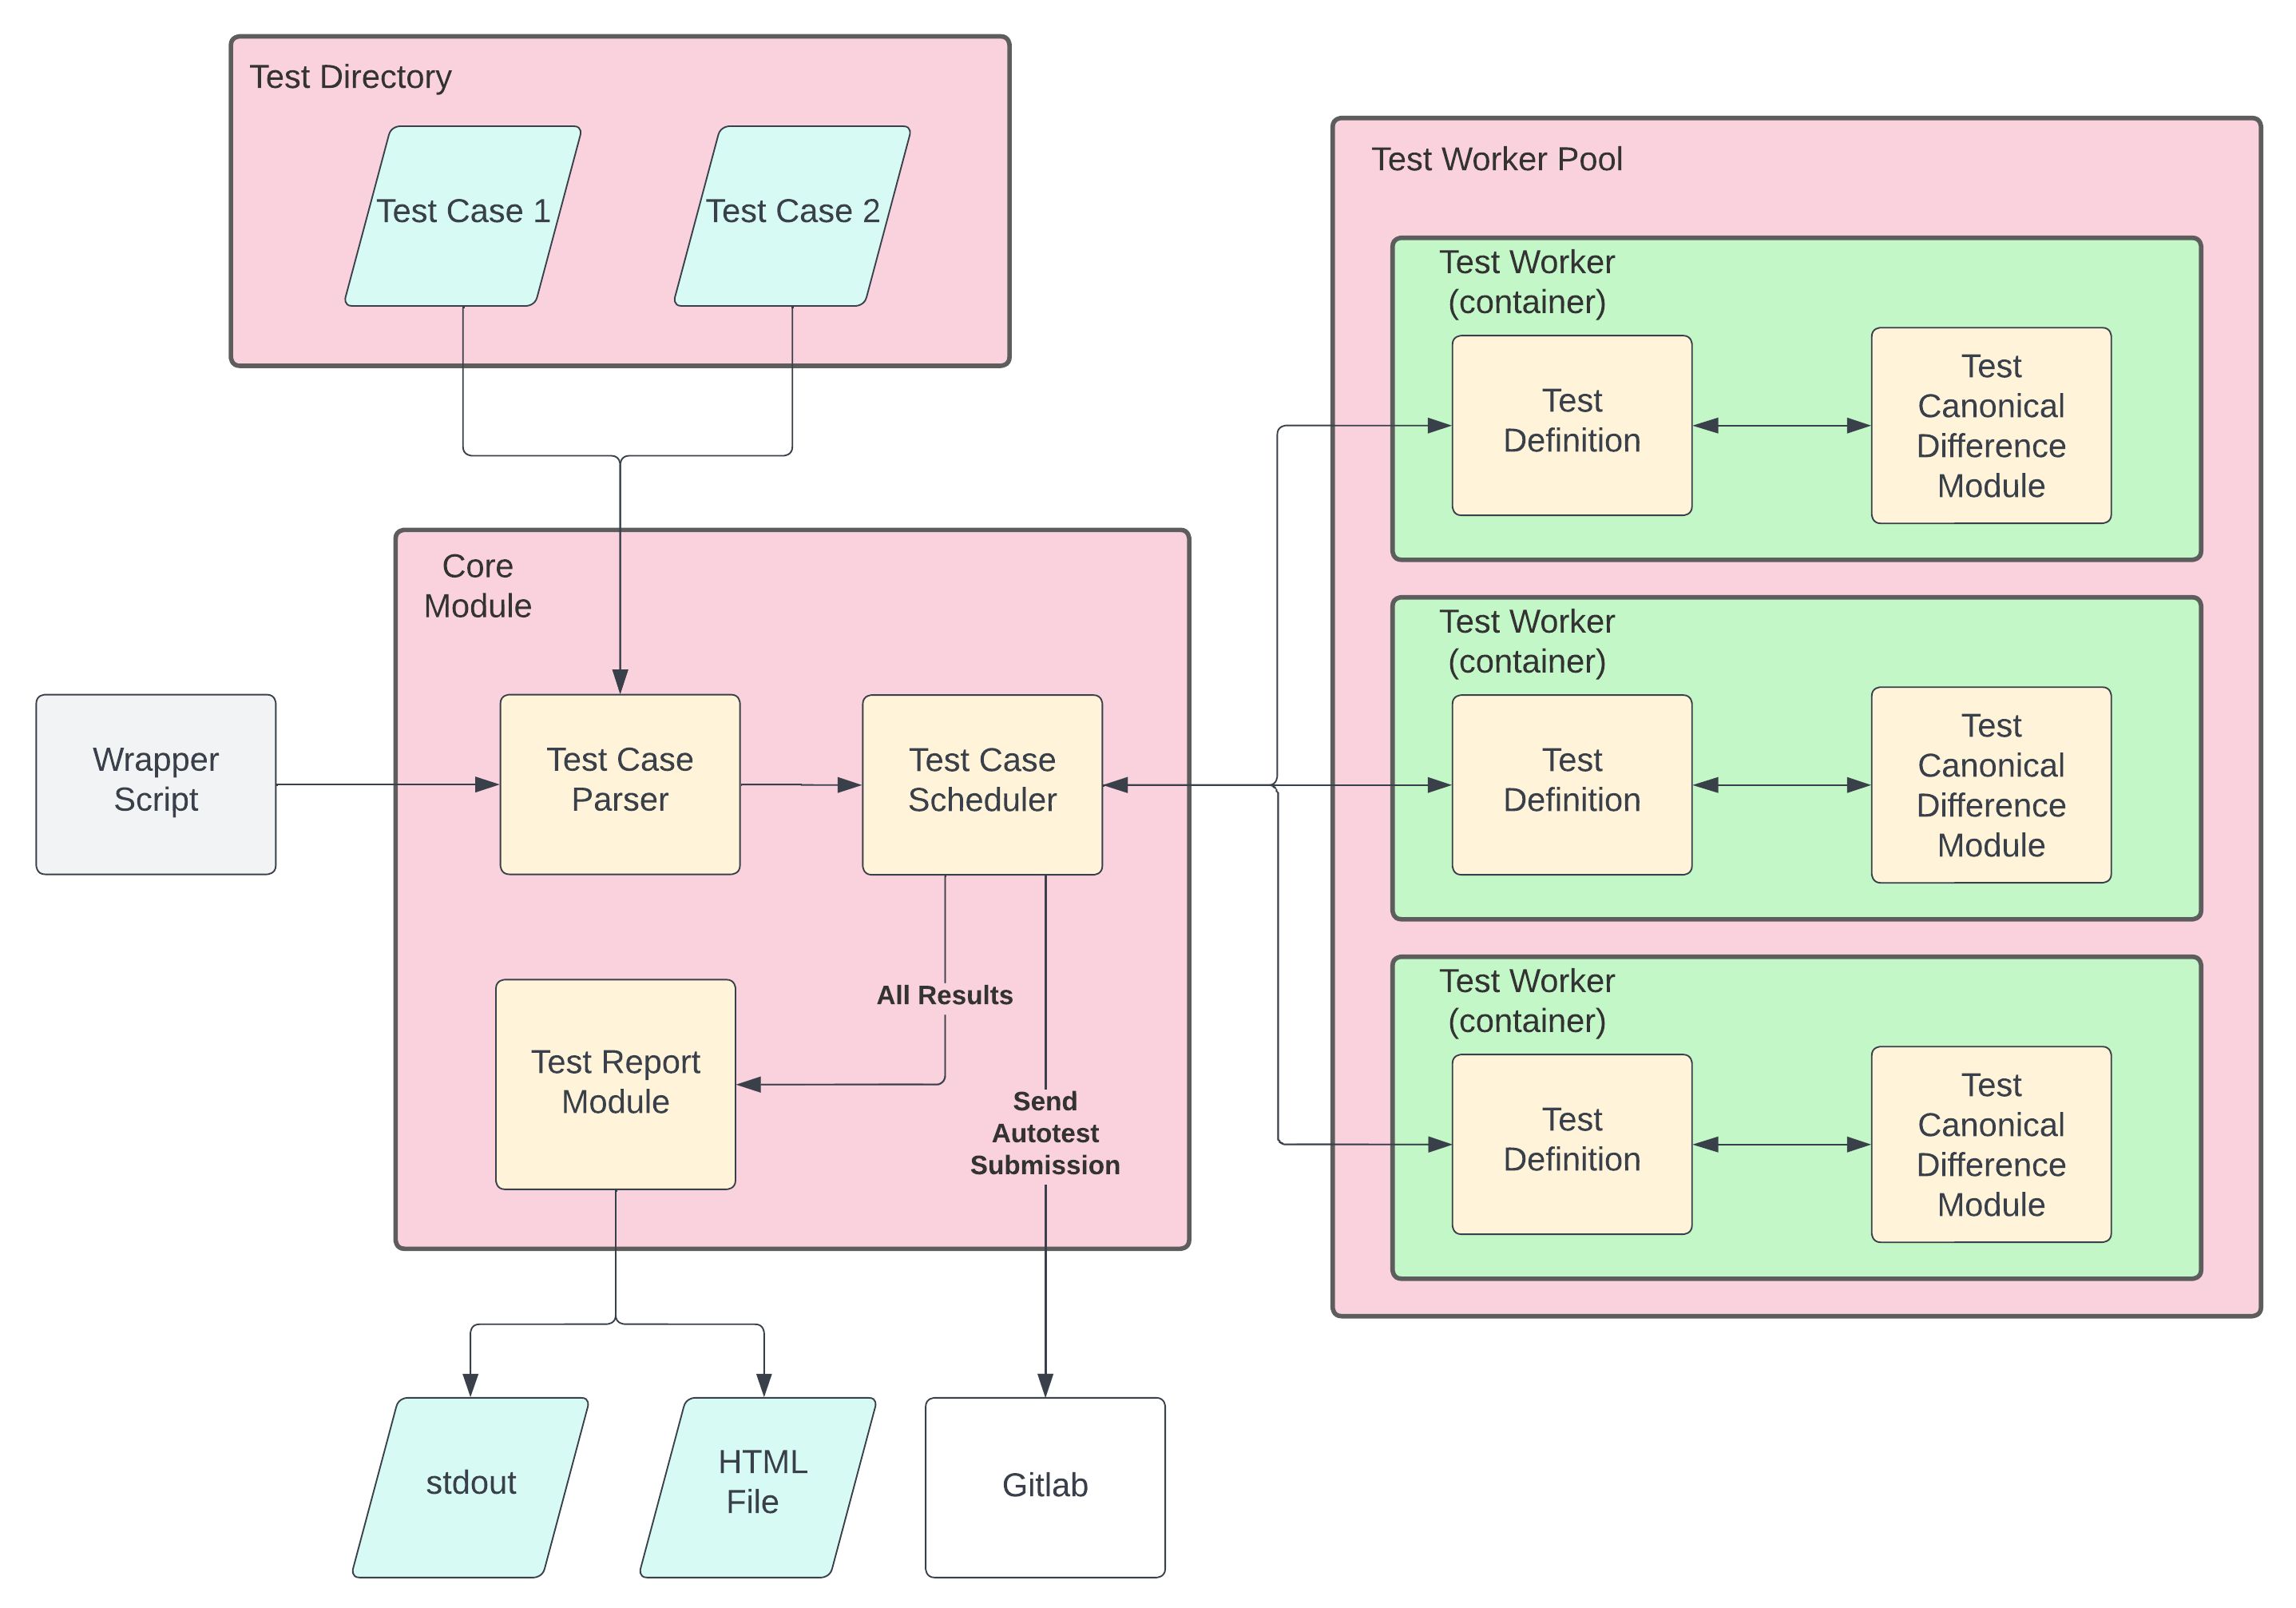
\includegraphics[width=1.25\textwidth, height=0.85\textheight, keepaspectratio=true,]{architecture}}
	\caption{Lemontest Core Architecture Diagram (incl. planned features)}
	\label{fig:architecture}
\end{figure}

\clearpage
\section{Modules}\label{modules}
From \autoref{fig:architecture}, we analyse the implementation of each module in order to understand how they work together in delivering the functionality of an automated marking tool. We also explore the additional functionality that has been introduced in \textit{lemontest} in order to fulfil the design requirements and achieve the thesis aims.

\subsection{Core Module}
The purpose of the \textit{core module} is to be the main controller of the code testing process and perform administrative tasks that do not warrant or are yet to be packaged into their own module. It achieves this by coordinating the execution of each of the modules within \textit{lemontest} and facilitating any information transfer required between them as shown in \autoref{fig:core_module_testing}. The main benefit of utilising a modular architecture is also visible where only abstractions of each module are exposed as interfaces. Abstracting the implementation of each module supports the long-term maintainability of \textit{lemontest} as changes would usually be isolated to the relevant module depending of the scope of the change. In the event that a module has been newly created or heavily rewritten, changes to the \textit{core module} itself would be minimal as long as the existing interface for each module has been fully implemented. To provide an easy transition between the old and new module implementations while providing a possible rollback plan, the constructor for the module can be simply switched to the new one (strategy pattern\footnote{Strategy is a behavioural design pattern that lets you define a family of algorithms, put each of them into a separate class, and make their objects interchangeable \cite{strategyPattern}.}).
\begin{figure}[h]
	\centering
	\begin{lstlisting}[language=python, breaklines=true, linewidth=\linewidth, tabsize=4]
def execute_autotest():
	# setup parser
	parser = Parser.Parser()
	# execute parser execution
	parser.parse_arguments()
	parser.parse_tests()
	parser.post_parse_misc()

	# setup test scheduler
	test_scheduler = TestScheduler.TestScheduler(parser.args(), parser.params())
	# schedule execute tests
	processed_tests = test_scheduler.schedule(parser.tests())
	# await execution finish and cleanup
	test_scheduler.cleanup()

	# report results
	# FIXME: Report Module (if necessary)
	failed_count = 0
	not_run_count = 0
	for test in processed_tests:
		print(test)
		if not test.passed():
			if not test.run_successful():
				not_run_count += 1
			else:
				failed_count += 1
			
	pass_str = f"{len(processed_tests) - failed_count - not_run_count} tests passed"
	fail_str = f"{failed_count} tests failed"
	if not_run_count:
		# two spaces before tests could not be run for some reason (autotest output parity)
		print(f"{pass_str} {fail_str}  {not_run_count} tests could not be run")
	else:
		print(f"{pass_str} {fail_str}")
	
	# TODO: perform administrative tasks here
	
	return 1 if failed_count + not_run_count else 0
	\end{lstlisting}
	\caption{Simplified version of the core module code which drives the code testing process}
	\label{fig:core_module_testing}
\end{figure}

\subsection{Parser Module}
The first step for the \textit{core module} is to initialise a \textit{parser module} which ingests \textit{lemontest} command-line parameters in order to retrieve the relevant \textit{lemontest} test specifications. The specifications are then processed into \textit{test case definitions} (described in \autoref{testCaseDef}) which are then made available to the \textit{core module}. Despite efforts to implement an entirely new version of the \textit{autotest} parser whilst maintaining backwards compatibility with existing test specifications, the original parsing process proved to be very complex and difficult to understand. There were also correctness concerns for the development of a new parser which would also need to be handled accordingly to meet the familiarity design goal.
With this difficulty in mind, it was noted that the existing \textit{autotest} parser already had reasonable performance for the majority of existing test specifications at UNSW CSE with negligible benefits expected from a new implementation \cite{parserConversation}.
As such, a new \textit{parser module} for \textit{lemontest} was deemed to be too time-consuming for this thesis. Instead, an adaptor\footnote{Adaptor is a structural design pattern that allows objects with incompatible interfaces to collaborate \cite{adaptorPattern}.} which abides with the module interface was implemented once the \textit{autotest} parser was isolated as much as possible which is shown in \autoref{fig:parserAdaptor}.
\begin{figure}[h]
	\centering
	\begin{lstlisting}[language=python, breaklines=true, linewidth=\linewidth, tabsize=4]
class Parser(AbstractParser):
    # standard vars
    _args = None
    _tests = None
    _params = None

    # getters
    def args(self):
        return self._args
    
    def tests(self):
        return self._tests
    
    def params(self):
        return self._params

    # argument and test parsing functionality

    # literally a reordering of the original autotest parser but done in a way
    # that made some sense (and was easier to work with)
    # ... removed extraneous commenting ...
    def parse_arguments(self):
        self._args = cmdlineargs.parse_arguments()

    def parse_tests(self):
        test_specification_pathname = cmdlineargs.find_test_specification(self._args)
        tests_as_dicts, self._params = parsetestspec.parse_file(
            test_specification_pathname,
            initial_parameters=self._args.initial_parameters,
            initial_tests=self._args.initial_tests,
            debug=self._args.debug,
        )
        # god knows why it's done like this but it's necessary for normalisation
        self._tests = dict(
            (label, Test(self._args.autotest_directory, **t))
            for (label, t) in tests_as_dicts.items()
        )

    def post_parse_misc(self):
        cmdlineargs.normalize_arguments(self._args, self._tests)
        # make the tests actually usable (convert dict to list)
        # get tests to run based on label selection
        self._tests = [test for (label, test) in self._tests.items() if label in self._args.labels]
	\end{lstlisting}
	\caption{Adaptor code porting existing autotest test case parser to lemontest}
	\label{fig:parserAdaptor}
\end{figure}

\subsection{Test Case Definition}\label{testCaseDef}
The \textit{test case definition} is a template for which all information necessary for a test case and its execution is stored. This includes but is not limited to information such as required files, pre-checks, setup instructions, execution instructions and the expected behaviour for the test. The \textit{test case definition} can also be executed to perform the test which will be further described within the \textit{worker module} at \autoref{testWorker}. \autoref{fig:testDefinition} shows the abstract interface that is implemented by the module with the concrete implementation available in the \textit{lemontest} project repository.
\begin{figure}[h]
	\centering
	\begin{lstlisting}[language=python, breaklines=true, linewidth=\linewidth, tabsize=4]
class AbstractTest:
    """
    Abstract test class
    """

    def __init__(self):
        """
        Initialise a test
        You will need to create a test on initialisation
        since it will be easiest to work with test instances

        Returns: None
        """
        pass


    def __str__(self):
        """
        Return a string instatiation of a test

        Returns: str
        """
        pass


    def preprocess(self):
        """
        Execute any preprocessing such as checks etc.
        Should return whether preprocessing succeded
        
        NOTE: This function will most likely contain critical sections
        Ensure critical section safety with synch primitives (mutex lock etc.)

        Returns: bool
        """
        pass


    def run_test(self):
        """
        Execute the test
        Should return whether the test executed successfully

        Returns: bool
        """
        pass


    def postprocess(self):
        """
        Executes any postprocessing such as sanitisation etc.
        Should return whether postprocessing succeded

        Returns: bool
        """
        pass
    # ... more functions below
	\end{lstlisting}
	\caption{Simplified test case definition abstract interface}
	\label{fig:testDefinition}
\end{figure}

\subsection{Test Case Scheduler Module}
Once \textit{test case definitions} have been created by the \textit{parser module}, the \textit{core module} will then initialise the \textit{scheduler module} to allocate the definitions to a pool of \textit{test workers} (detailed in \autoref{testWorker}) for processing. Each worker is initialised and managed by the \textit{scheduler module} as shown in \autoref{fig:testSchedulerInit}. The \textit{scheduler module} also manages any resources that are shared within the pool and returns processed \textit{test case definitions} back to the \textit{core module} as seen in \autoref{fig:testSchedulerWorker} and \autoref{fig:testSchedulerSchedule}. By taking advantage of the Python \textit{multiprocessing} package, the \textit{scheduler module} is able to provide \textit{lemontest} the ability to execute tests in parallel rather than exclusively in serial which is described in \autoref{autotestLimitations} as a major limitation of \textit{autotest}.
\begin{figure}[h]
	\centering
	\begin{lstlisting}[language=python, breaklines=true, linewidth=\linewidth, tabsize=4]
def __init__(self, args: Namespace, parameters: Dict[str, Any]):
    self.args = args
    self.parameters = parameters
    self.shared_dir = Path(tempfile.mkdtemp())
    atexit.register(lambda: shutil.rmtree(self.shared_dir))
    self.colored = (
        termcolor_colored
        if parameters["colorize_output"]
        else lambda_function
    )
    try:
        # set the fork start method
        set_start_method('fork')
        # spawn Lock for test preprocessing shared directory access
        pLock = Lock()
        # spawn worker pool
        self.worker_pool = Pool(initializer=test_worker_init, initargs=(pLock,), processes=self.parameters["worker_count"], maxtasksperchild=1)
        # cleanup worker pool at exit (fixes issue with lemontest exiting without fully terminating processes)
        atexit.register(self.cleanup)
    except Exception as err:
        die(err)
	\end{lstlisting}
	\caption{Test case scheduler initialisation code to setup worker pool and shared resources}
	\label{fig:testSchedulerInit}
\end{figure}
\begin{figure}[h]
	\centering
	\begin{lstlisting}[language=python, breaklines=true, linewidth=\linewidth, tabsize=4]
# setup a global variable to inherit a global lock for the test preprocessing
# see: test_worker to see why this is absolutely necessary
# we can't use multiprocessing.Manager because that will break if we
# isolate networking within the sandbox (more common than not)
def test_worker_init(lock: Lock) -> None:
    global pLock
    pLock = lock


# initalise worker and execute task
def test_worker(test: AbstractTest, shared_dir: Path, parameters) -> AbstractTest:
    worker = TestWorker(shared_dir, **parameters)
    worker.setup()
    res = worker.execute(test, pLock) #pLock available from Pool initializer (global var)
    worker.cleanup()
    return res
	\end{lstlisting}
	\caption{Test case worker code including measures to introduce a shared mutex lock}
	\label{fig:testSchedulerWorker}
\end{figure}
\begin{figure}[h]
	\centering
	\begin{lstlisting}[language=python, breaklines=true, linewidth=\linewidth, tabsize=4]
def schedule(self, tests: List[AbstractTest]) -> List[AbstractTest]:
    # process tests to be run
    tests = [(test, self.shared_dir, self.parameters) for test in tests]

    # FIXME: compile.sh and runtests.pl was executed here usually

    # copy required files (student submission + test provided)
    # into a known temp directory from scheduler
    copy_files_to_directory(self.shared_dir, self.parameters, self.args)

    # check tests to ensure we have all files in the shared_dir to execute tests, otherwise die with missing files
    req_files_set = set.intersection(
        *[set(test.params()["files"]) for (test, _, _) in tests]
    )
    # FIXME: root_dir argument is only available in python 3.10
    # CSE at time of writing is on version 3.9 => have to do things the old fashioned way
    orig_dir = os.getcwd()
    os.chdir(self.shared_dir)
    missing_files = [f for f in req_files_set if not glob.glob(f)]
    if missing_files:
        die(f"Unable to run tests because these files were missing: {' '.join(missing_files)}")
    os.chdir(orig_dir)

    # schedule tests for execution (chunksize=1 necessary for proper containerisation)
    test_res = self.worker_pool.starmap(test_worker, tests, chunksize=1)

    # terminate worker pool as work is done
    self.worker_pool.terminate()
    self.worker_pool.join() # this doesn't sometimes work with .close() so just terminate

    # reset worker_pool in case cleanup gets triggered by signal
    self.worker_pool = None

    # return results
    return test_res
	\end{lstlisting}
	\caption{Simplified version of the test case scheduling code which assigns tests to the pool for processing}
	\label{fig:testSchedulerSchedule}
\end{figure}

\subsection{Test Worker Module}\label{testWorker}
The \textit{test worker} is a separate process initialised by the \textit{scheduler module} which will set up an exclusive area to execute a test that has been allocated to it independently of any other workers as shown in \autoref{fig:testWorkerExecute}. The \textit{test worker} also has an option to run the test within a sandbox environment (detailed in \autoref{sandboxContainer}) which will execute the test in a \textit{container} which is mostly isolated from the host system depending on the needs of the test.
\begin{figure}[h]
	\centering
	\begin{lstlisting}[language=python, breaklines=true, linewidth=\linewidth, tabsize=4]
def execute(self, test: AbstractTest, pLock: Lock):
    # this also allows us to cache on a shared binary resource
    # as such, we also consider test.preprocess() to be a critical section

    # rw bind in the scheduler temp directory (should allow caching between worker processes but must use lock)
    # available within Sandbox as "/shared" 
    # spawn sandbox runtime context
    with Sandbox(self.worker_root, self.shared_dir, **self.parameters) as sb:
        # run test preprocessing
        pLock.acquire()
        pStatus = test.preprocess(SHARED_DIR_DEST)
        pLock.release()
        if not pStatus:
            return test

        # execute test
        rStatus = test.run_test(SHARED_DIR_DEST)
        if not rStatus:
            return test

        # perform test postprocessing (output checking etc.)
        test.postprocess()

    # return processed test
    return test
	\end{lstlisting}
	\caption{Test worker code which executes a given test in a sandbox container}
	\label{fig:testWorkerExecute}
\end{figure}

\subsection{Sandbox Container}\label{sandboxContainer}
\textit{Sandbox} is a lightweight pure-Python container runtime implementation for Linux systems created specifically for \textit{lemontest} but can also be used in other applications. \textit{Sandbox} allows the executing process (Python interpreter) to execute code in a container similarly to \textit{chroot} but with extra features and sturdier protections in place.
Originally, the use of an industry standard container engine or existing project was considered but each was rejected with good cause:
\begin{itemize}
	\item Docker SDK for Python (Docker) \cite{docker-py}
	\begin{itemize}
		\item There is no documentation both on official and community sources on how a rootless container can be spun up.
		\item The \textit{test worker} process must be containerised itself as shown in \autoref{fig:testWorkerExecute} but no visibly easy way of performing this action was discovered without introducing avoidable overhead such as the need to close and re-open the \textit{test worker} process within the new container.
		\item Rootless installation is possible but is entirely user managed which can lead to issues with inexperienced users.
	\end{itemize}
	\item Furnace \cite{furnace}
	\begin{itemize}
		\item Requires root privileges due to reliance on \textit{setns} system call.
		\item Easy to use interface shown in \autoref{fig:furnace} influenced how \textit{Sandbox} was designed.
	\end{itemize}
	\item Pocket \cite{pocket}
	\begin{itemize}
		\item Similar issues to Docker but is entirely rootless and did not rely on \textit{setns}.
		\item Avoidance of \textit{setns} guided how \textit{Sandbox} would do the same.
	\end{itemize}
\end{itemize}
\begin{figure}[h]
	\centering
	\begin{lstlisting}[language=python, breaklines=true, linewidth=\linewidth, tabsize=4]
from furnace.context import ContainerContext

with ContainerContext('/opt/ChrootMcChrootface') as container:
    container.run(['ps', 'aux'])
	\end{lstlisting}
	\caption{Furnace container listing processes with a arbitrary root location set}
	\label{fig:furnace}
\end{figure}
As no existing container engine or implementation met all the requirements set by \textit{lemontest}, \textit{Sandbox} was created to deliver containerisation functionality as shown in \autoref{fig:testWorkerExecute}. At a high level, \textit{Sandbox} allows Python code to be run in a container by performing the following:
\begin{enumerate}
	\item Python code imports and uses the Sandbox context to execute containerised code (\autoref{fig:sandboxContext}).
	\begin{figure}[h]
		\centering
		\begin{lstlisting}[language=python, breaklines=true, linewidth=\linewidth, tabsize=4]
with Sandbox(<sandbox root>, <shared directory if any>, <sandbox parameters>) as sb:
	# code to be executed
		\end{lstlisting}
		\caption{Sandbox context manager}
		\label{fig:sandboxContext}
	\end{figure}
	\item Sandbox and associated PID 1\footnote{A process running as PID 1 inside a container is treated specially by Linux} manager instance is initialised.
	\item User namespace of the Python process is isolated from the host which is remapped for the process to see itself as possessing root privileges (\autoref{fig:sandboxUser}).
	\begin{figure}[h]
		\centering
		\begin{lstlisting}[language=python, breaklines=true, linewidth=\linewidth, tabsize=4]
def unshare_user():
    # uid & gid mapping
    uid = os.getuid()
    gid = os.getgid()

    uidmapfile = f"/proc/self/uid_map"
    gidmapfile = f"/proc/self/gid_map"
    setgroupsfile = f"/proc/self/setgroups"
    uidmap = f"0 {uid} 1"
    gidmap = f"0 {gid} 1"

    # unshare user namespace
    libc.unshare(libc.CLONE_NEWUSER)

    # write uid & gid mapping
    # user_namespaces(7)
    # The data written to uid_map (gid_map) must consist of a single line that
    # maps the writing process's effective user ID (group ID) in the parent
    # user namespace to a user ID (group ID) in the user namespace.
    with open(uidmapfile, "w") as uidmap_f:
        uidmap_f.write(uidmap)

    # user_namespaces(7)
    # In the case of gid_map, use of the setgroups(2) system call must first
    # be denied by writing "deny" to the /proc/[pid]/setgroups file (see
    # below) before writing to gid_map.
    with open(setgroupsfile, "w") as setgroups_f:
        setgroups_f.write("deny")    
    with open(gidmapfile, "w") as gidmap_f:
        gidmap_f.write(gidmap)
		\end{lstlisting}
		\caption{Simplified version of Sandbox user namespace isolation and remapping code}
		\label{fig:sandboxUser}
	\end{figure}
	\item PID namespace of the Python process is isolated with the process no longer able to see other processes running on the host except for itself.
	\item Python process is forked with the child process executing as PID 1 which inherits control while the parent is killed (\autoref{fig:sandboxFork}).
	\begin{figure}[h]
		\centering
		\begin{lstlisting}[language=python, breaklines=true, linewidth=\linewidth, tabsize=4]
# fork python interpreter into child process to be PID 1
self.pid = os.fork()

# child process (PID 1)
if self.pid == 0:
    # instantiate and execute PID1 setup as everything
    # from now on spawns from this process
    self.pid1_class = pid1.PID1(self.root_dir, self.isolate_networking, self.debug, self.bind_mounts)
    self.pid1_class.run()
# wait then kill parent process which doesn't have pid 1
# child process is PID1 so we're safe as all control gets inherited back
else:
    # don't execute any exit handlers
    os._exit(0)
		\end{lstlisting}
		\caption{Sandbox fork to ensure Python process is PID 1 with original parent killed}
		\label{fig:sandboxFork}
	\end{figure}
	\item Python process that is now PID 1 runs PID 1 related setup such as zombie process reaping with the remaining namespaces also isolated as necessary (cgroups, IPC, mount, network etc.).
	\item Sandbox container file system such as directories and devices are set up via bind mounts after pivoting root to a predefined sandbox root directory (\autoref{fig:sandboxRun}).
	\begin{figure}[h]
		\centering
		\begin{lstlisting}[language=python, breaklines=true, linewidth=\linewidth, tabsize=4]
def run(self):
    self.enable_zombie_reaping()
    unshare_process(self.isolate_networking)
    self.setup_root_mount()
    self.mount_defaults()
    self.create_default_dev_nodes()
    self.umount_old_root()
		\end{lstlisting}
		\caption{Sandbox code to enable zombie reaping and setup of container file system}
		\label{fig:sandboxRun}
	\end{figure}
	\item Sandbox has now been setup and Python code that was to be executed in the container is run.
	\item Sandbox cleans up the container and reverts root for the Python process to the pre-container directory.
	\item As root privilege is required for \textit{setns}, it is not possible for the Python process to reset the namespace to what is was pre-container without root. This severely limits what is possible for the Python process after a Sandbox container has been used but this is of little relevance when used with \textit{lemontest} (\autoref{fig:testWorkerExecute}).
\end{enumerate}

\subsection{Test Case Canonical Difference Module}
As part of the post-processing of a test, recall from the background that the side-effects of the test must be checked to determine if a test has passed or failed. If all side-effects match the expected, the test has passed and no further action is taken. However, an explanation into what went wrong must be generated by the \textit{canonical difference module} if the test fails. In order to best follow the output of the original \textit{autotest}, much of the process has been ported over with changes made to fit the process to the architecture as best as possible. As all possible side-effects including files are checked within this module, it must be performed within the container if one is used and before the contents of the test directory is deleted. This has led to the \textit{canonical difference module} being more coupled with the \textit{test definition} than other module combinations but I believe it is the best solution at the current time. At a high level, the process of the \textit{canonical difference module} works as follows:
\begin{enumerate}
	\item A test which can comprise of multiple sub-tests is executed with each sub-test processing their own ``short explanation" if something were to not match what is expected such as ``output not matching" without further detail (\autoref{fig:testShort}).
	\begin{figure}[h]
		\centering
		\begin{lstlisting}[language=python, breaklines=true, linewidth=\linewidth, tabsize=4]
def run_individual_test(self):
    # update environment if not set
    # not usually necessary so disable if not providing any benefit
    self.set_environ()

	# execute sub-test
    (stdout, stderr, self.returncode) = run(**self.parameters)   
    self.stdout = stdout
    self.stderr = stderr

    # checks for any issues in stdout or stderr and/or files
    self.process_short_explanation()
    # the test passes if there is no explanation for the error
    self.test_passed = not self.short_explanation

    # NOTE: skip any long explanation processing till postprocessing and only do it if necessary
		\end{lstlisting}
		\caption{Simplified test worker code checking sub-test side-effects and generating a short explanation if necessary}
		\label{fig:testShort}
	\end{figure}
	\item Once all sub-tests are executed and short explanations generated, test post-processing begins. If all sub-tests have passed, there is an early exit once the overall test passed status has been set to true.
	\item In the event that one or more sub-tests have failed, the best failed sub-test to report is chosen and a long explanation for the sub-test is generated which provides more detail on the nature of the failure such as where and how the side-effects differ when compared to what is expected.
	\item Both the short and long explanation of the selected failed sub-test are then inherited by overall test (\autoref{fig:testLong}).
	\begin{figure}[h]
		\centering
		\begin{lstlisting}[language=python, breaklines=true, linewidth=\linewidth, tabsize=4]
def postprocess(self):
    # determine if we have passed all individual tests
    failed_individual_tests = [it for it in self.individual_tests if not it.passed()]
    self.test_passed = not failed_individual_tests
    # early exit if we have passed all individual tests
    if self.test_passed:
        self.stdout = self.individual_tests[0].stdout
        self.stderr = self.individual_tests[0].stderr
        return

    # pick the best failed test to report
    # if we have errors then should be more informative than incorrect output except memory leaks
    if not failed_individual_tests[-1].stderr_ok and (
        not self.parameters["unicode_stderr"]
        or ("free not called" not in failed_individual_tests[-1].stderr)
    ):
        individual_test = failed_individual_tests[-1]
    else:
        individual_test = failed_individual_tests[0]

    self.stdout = individual_test.stdout
    self.stderr = individual_test.stderr
    self.short_explanation = individual_test.short_explanation
    self.long_explanation = individual_test.get_long_explanation()
		\end{lstlisting}
		\caption{Test worker code checking if any sub-tests failed and generating a long explanation for the ``best" sub-test if necessary which is then inherited by the overall test}
		\label{fig:testLong}
	\end{figure}
\end{enumerate}
\subsection{Test Case Report Module}
Once all tests have been processed through the \textit{scheduler module}, the \textit{core module} will report the findings of each test to the user in a format that is almost identical to the \textit{original} autotest. Originally, the \textit{report module} was to provide the ability for users to receive results on the terminal like with \textit{autotest} but also as a HTML file which would assist readability. Due to time constraints, the HTML feature was dropped but the terminal output feature has been kept (\autoref{fig:core_module_testing}).

\clearpage
\section{Example Demonstration (COMP1521 float\_2048)}
For the thesis demonstration, and to evaluate the new implementation, we have a small example execution of \textit{lemontest} in action with the \textit{float\_2048} exercise from the UNSW CSE COMP1521 \textit{Computer Systems Fundamentals} course.

\subsection{Environment}
The demonstration environment consists as follows:
\begin{itemize}
	\item UNSW CSE \textit{nw-k17-login1} server which hosts dependencies of the test and \textit{lemontest} such as \textit{python}, \textit{dcc}, \textit{c\_check} and \textit{tqdm} (\textit{lemontest} requires >= Python 3.9).
	\item An installation of \textit{lemontest} which is a directory containing of the cloned project repository.
	\item An executable wrapper script that points to the \textit{lemontest} installation, preloads the relevant parameters and passes the users choice of test to \textit{lemontest} (\autoref{fig:wrapper}).
	\begin{figure}[h]
		\centering
		\begin{lstlisting}[language=bash, breaklines=true, linewidth=\linewidth, tabsize=4]
#!/bin/sh

parameters="
	dcc_output_checking = 0
	default_compilers = {'c': [['dcc', '-fsanitize=address'], ['dcc', '-fsanitize=valgrind']]}
	default_checkers = {'c': [['1521', 'c_check']], 's' : [['1521', 'mipsy', '--check']]}
"

exec ../lemontest.py --exercise_directory ../tests --parameters "$parameters" "$@"
		\end{lstlisting}
		\caption{Wrapper script for lemontest assuming the installation and test directory is in the parent directory}
		\label{fig:wrapper}
	\end{figure}
	\item A \textit{float\_2048.c} file which can be either correct or incorrect to the specification.
\end{itemize}
Although the \textit{lemontest} installation can be placed in any directory accessible by the user, the wrapper script should be located in the same directory as the \textit{float\_2048.c} file. The wrapper script can also be placed in a directory that is within the PATH but for this example, both the wrapper and C file are located in the same directory (\autoref{fig:demoFiles}).
\begin{figure}[h]
	\centering
	\begin{lstlisting}[breaklines=true, linewidth=\linewidth, tabsize=4]
z5208931@nw-k17-login1:~lemontest/demo$ ls -l
total 8
-rw-r----- 1 z5208931 z5208931 1962 Nov 18 14:25 float_2048.c
-rwxr-x--- 1 z5208931 z5208931  314 Nov 17 20:17 wrapper.sh
	\end{lstlisting}
	\caption{Wrapper script for lemontest assuming the installation and test directory is in the parent directory}
	\label{fig:demoFiles}
\end{figure}

\subsection{Execution}
Within the folder containing the wrapper and C file, \textit{lemontest} can be invoked to test the given \textit{float\_2048.c} file as follows where \textit{1521\_float\_2048} is the directory name containing the relevant test specification:
\begin{lstlisting}[breaklines=true, linewidth=\linewidth, tabsize=4]
z5208931@nw-k17-login1:~lemontest/demo$ ./wrapper.sh 1521_float_2048
\end{lstlisting}
It is also noted that the specification has been modified from the pre-existing \textit{autotest} version to include \textit{lemontest} specific parameters (\autoref{fig:floatTestSpec}).
\begin{figure}[h]
	\centering
	\begin{lstlisting}[breaklines=true, linewidth=\linewidth, tabsize=4]
max_cpu=30
worker_count=4 # added to ensure lemontest runs with 4 test workers in the pool
worker_read_only_mount=["/home/cs1521", "/web/cs1521"] # added to ensure dcc and c_check are visible in the container
compiler_args=-Dmain=_main autotest_float_2048.c float_2048.c -o float_2048
files=float_2048.c

0 command=./float_2048 8 expected_stdout="16384\n"
1 command=./float_2048 3.99 expected_stdout="8171.52002\n"
2 command=./float_2048 0.748 expected_stdout="1531.90405\n"
3 command=./float_2048 -0.749 expected_stdout="-1533.95203\n"
4 command=./float_2048 4.298765432e-31 expected_stdout="8.80387163e-28\n"
5 command=./float_2048 9.91234567e+37 expected_stdout="inf\n"
6 command=./float_2048 inf expected_stdout="inf\n"
7 command=./float_2048 -inf expected_stdout="-inf\n"
8 command=./float_2048 0.0 expected_stdout="0\n"
9 command=./float_2048 -0.0 expected_stdout="-0\n"
10 command=./float_2048 NaN expected_stdout="nan\n"
	\end{lstlisting}
	\caption{float\_2048 autotest specification including lemontest specific parameters}
	\label{fig:floatTestSpec}
\end{figure}
\subsection{Execution Results}\label{lemontestResults}
Depending on if the user provided \textit{float\_2048.c} is correct or has issues, the following 3 scenarios are the most likely to be encountered:
\begin{itemize}
	\item The provided program is correct (\autoref{fig:floatTestCorrect}).
	\item The provided program is incorrect with a logic error such as only multiplying by 1024 (\autoref{fig:floatTestIncorrect}).
	\item The provided program is incorrect with a segmentation fault error (\autoref{fig:floatTestSegfault}).
\end{itemize}
\begin{figure}[h]
	\centering
	\begin{lstlisting}[breaklines=true, linewidth=\linewidth, tabsize=4]
Ran 11 tests | 11 tests passed | 0 tests failed: 100%|███████████████████████████████| 11/11 [00:05<00:00,  2.16 test/s]
Test 0 (./float_2048 8) - passed
Test 1 (./float_2048 3.99) - passed
Test 2 (./float_2048 0.748) - passed
Test 3 (./float_2048 -0.749) - passed
Test 4 (./float_2048 4.298765432e-31) - passed
Test 5 (./float_2048 9.91234567e+37) - passed
Test 6 (./float_2048 inf) - passed
Test 7 (./float_2048 -inf) - passed
Test 8 (./float_2048 0.0) - passed
Test 9 (./float_2048 -0.0) - passed
Test 10 (./float_2048 NaN) - passed
11 tests passed 0 tests failed
	\end{lstlisting}
	\caption{Lemontest output with correct float\_2048.c submission}
	\label{fig:floatTestCorrect}
\end{figure}
\begin{figure}[h]
	\centering
	\begin{lstlisting}[breaklines=true, linewidth=\linewidth, tabsize=4]
Ran 11 tests | 6 tests passed | 5 tests failed: 100%|████████████████████████████████| 11/11 [00:05<00:00,  2.17 test/s]
Test 0 (./float_2048 8) - failed (Incorrect output)
Your program produced this line of output:
8192

The correct 1 lines of output for this test were:
16384

The difference between your output(-) and the correct output(+) is:
- 8192
+ 16384
You can reproduce this test by executing these commands:
  dcc -fsanitize=address -Dmain=_main autotest_float_2048.c float_2048.c -o float_2048
  ./float_2048 8

Test 1 (./float_2048 3.99) - failed (Incorrect output)
Your program produced this line of output:
4085.76001

The correct 1 lines of output for this test were:
8171.52002

The difference between your output(-) and the correct output(+) is:
- 4085.76001
+ 8171.52002
You can reproduce this test by executing these commands:
  dcc -fsanitize=address -Dmain=_main autotest_float_2048.c float_2048.c -o float_2048
  ./float_2048 3.99

... removed some tests that failed to fit on one page ...

Test 5 (./float_2048 9.91234567e+37) - passed
Test 6 (./float_2048 inf) - passed
Test 7 (./float_2048 -inf) - passed
Test 8 (./float_2048 0.0) - passed
Test 9 (./float_2048 -0.0) - passed
Test 10 (./float_2048 NaN) - passed
6 tests passed 5 tests failed
	\end{lstlisting}
	\caption{Lemontest output with incorrect float\_2048.c submission (multiplying by 1024)}
	\label{fig:floatTestIncorrect}
\end{figure}
\begin{figure}[h]
	\centering
	\begin{lstlisting}[breaklines=true, linewidth=\linewidth, tabsize=4]
Ran 11 tests | 5 tests passed | 6 tests failed: 100%|████████████████████████████████| 11/11 [00:27<00:00,  2.48s/ test]
Test 0 (./float_2048 8) - failed (errors)
Your program produced these errors:

float_2048.c:31:9: runtime error - store to misaligned address 0x0000deadbeef for type 'int', which requires 4 byte alignment
Execution stopped in float_2048(bits=1090519040) in float_2048.c at line 31:

uint32_t float_2048(uint32_t bits) {
    float_components_t f = float_to_components(bits);

    if (f.exponent != 0 && f.exponent != EXPONENT_INF_NAN) {
        // if we have a normal non-zero number increase the exponent
-->     *(int *)0xdeadbeef = 42;
        f.exponent += 11;

        if (f.exponent >= EXPONENT_INF_NAN) {

Values when execution stopped:

bits = 1090519040
f = {sign = 0, exponent = 130, fraction = 0}

Function Call Traceback
float_2048(bits=1090519040) called at line 18 of autotest_float_2048.c
main(argc=2, argv=0x7fff5abe0e58)
You can reproduce this test by executing these commands:
  dcc -fsanitize=address -Dmain=_main autotest_float_2048.c float_2048.c -o float_2048
  ./float_2048 8

... removed some tests that failed to fit on one page ...

Test 6 (./float_2048 inf) - passed
Test 7 (./float_2048 -inf) - passed
Test 8 (./float_2048 0.0) - passed
Test 9 (./float_2048 -0.0) - passed
Test 10 (./float_2048 NaN) - passed
5 tests passed 6 tests failed
	\end{lstlisting}
	\caption{Lemontest output with incorrect float\_2048.c submission and dcc compiler (segmentation fault)}
	\label{fig:floatTestSegfault}
\end{figure}
These reports from \textit{lemontest} are almost identical to that of the original \textit{autotest} with the changes being related to the parallelised nature of test execution with \textit{lemontest} (\autoref{fig:floatAutotest}).
\begin{figure}[h]
	\centering
	\begin{lstlisting}[breaklines=true, linewidth=\linewidth, tabsize=4]
1521 c_check float_2048.c
dcc -fsanitize=address -Dmain=_main autotest_float_2048.c float_2048.c -o float_2048
dcc -fsanitize=valgrind -Dmain=_main autotest_float_2048.c float_2048.c -o float_2048
Test 0 (./float_2048 8) - passed
Test 1 (./float_2048 3.99) - passed
Test 2 (./float_2048 0.748) - passed
Test 3 (./float_2048 -0.749) - passed
Test 4 (./float_2048 4.298765432e-31) - passed
Test 5 (./float_2048 9.91234567e+37) - passed
Test 6 (./float_2048 inf) - passed
Test 7 (./float_2048 -inf) - passed
Test 8 (./float_2048 0.0) - passed
Test 9 (./float_2048 -0.0) - passed
Test 10 (./float_2048 NaN) - passed
11 tests passed 0 tests failed
	\end{lstlisting}
	\caption{Autotest output with correct float\_2048.c submission}
	\label{fig:floatAutotest}
\end{figure}

\clearpage
\section{Best Practices (Technical Debt Management)}
In addition to the technical implementation of \textit{lemontest}, multiple best practices have been implemented with \textit{lemontest} to deliver on the thesis goals. We will explore the major practices undertaken for \textit{lemontest} which include project management, code documentation and regression testing.

\subsection{Project Management}
Any serious project expecting multiple contributors should employ project management tools such as version control and issue tracking to support contributors with features that improve quality of life during development. With \textit{lemontest}, the project is hosted on GitHub which utilises \textit{git} to perform version control for contributors. GitHub also provides issue tracking and continuous integration/continuous delivery via the GitHub Issues and GitHub Actions services respectively. The issue tracking service allow users to report issues and bugs with \textit{lemontest} to the repository directly which is of particular importance as future development of \textit{lemontest} continues.
The \textit{lemontest} GitHub repository can be viewed at \url{https://github.com/hexDoor/lemontest}.

\subsection{Code Documentation}
Recall from the \textit{autotest limitations} (\autoref{autotestLimitations}) that the lack of in-depth documentation of the code has been an issue for contributors. The release version of \textit{lemontest} as shown in the code examples within \autoref{modules} have significant commenting on all important code which will assist contributors in understanding what the code is doing. In addition to the documentation already provided by the original \textit{autotest} which remains mostly the same with \textit{lemontest}, documentation on any \textit{lemontest} exclusive features have also been made available (\autoref{fig:docsLemontestParams}).
\begin{figure}[h]
	\centering
	\makebox[\textwidth][c]{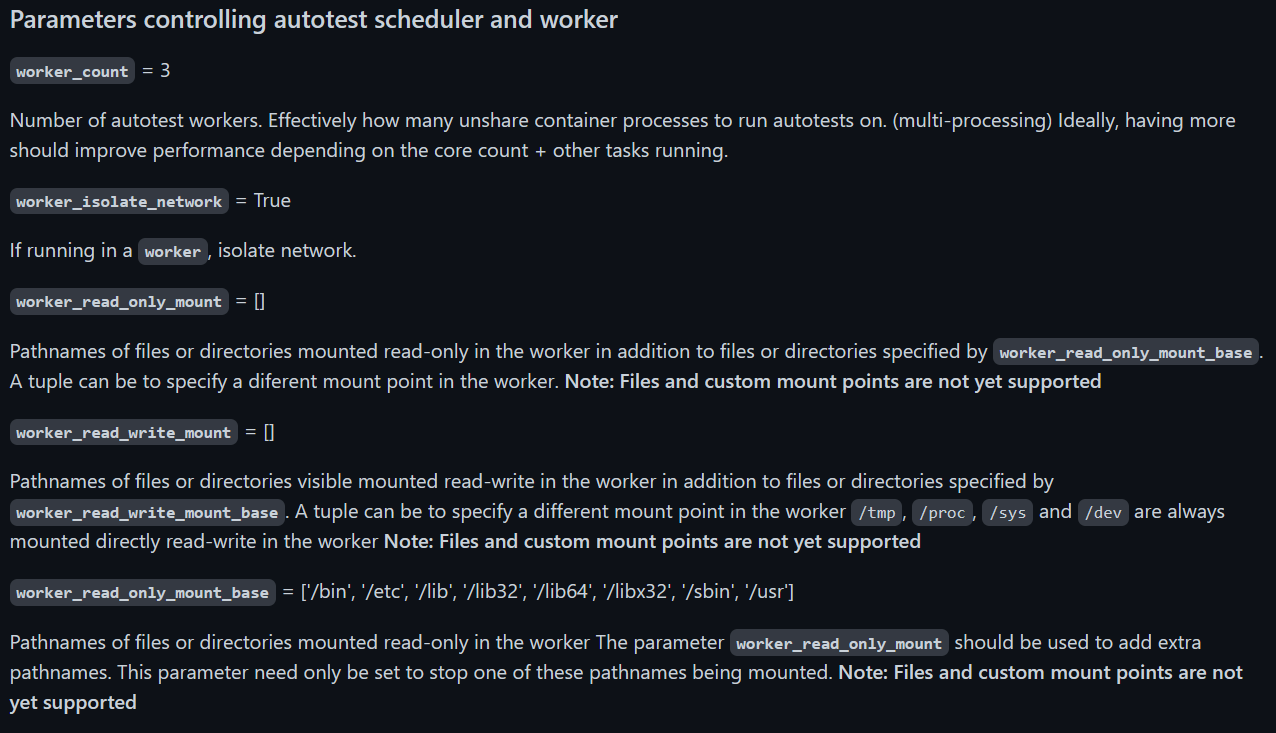
\includegraphics[width=\textwidth, height=0.85\textheight, keepaspectratio=true,]{paramdocs}}
	\caption{Parameter documentation on lemontest exclusive parameters}
	\label{fig:docsLemontestParams}
\end{figure}

\subsection{Regression Testing}
My previous work with \textit{autotest} involved porting the regression tests from a shell script into \textit{pytest} cases. It would have been ideal to provide more concrete test cases, but time constraints prevented these improvements from being made. As such, the pre-existing regression testing has been carried over to \textit{lemontest} with all current \textit{pytest} cases passing with the release version of \textit{lemontest} (\autoref{fig:pytest}).

\begin{figure}[h]
	\centering
	\begin{lstlisting}[breaklines=true, linewidth=\linewidth, tabsize=4]
======================= test session starts ======================
platform linux -- Python 3.10.6, pytest-7.2.0, pluggy-1.0.0
rootdir: /home/z5208931/lemontest
collected 14 items

pytest/test_standard.py ..............                      [100%]

======================= 14 passed in 2.99s =======================
	\end{lstlisting}
	\caption{Lemontest pytest output}
	\label{fig:pytest}
\end{figure}

\unchapter{6}{Evaluation}
With \textit{lemontest} complete for this thesis, as well as the example execution from the thesis demonstration, we can now compare \textit{lemontest} against the design goals detailed earlier.

\section{Maintainability}
The maintainability design goal is stated as: \textit{The design should be adequately documented, support an ease of maintainability and possible extension of features via the appropriate architectural decisions.}

As supported by the modular architecture and significant code documentation of \textit{lemontest} detailed in \autoref{architecture}, the goal has been met and can be seen as a significant improvement over the existing \textit{autotest}.

\textit{Lemontest} may fall short in some modules such as the \textit{parser module} and \textit{canonical difference module} which require further work to solve their respective limitations that was not viable to complete within the thesis time frame.

Despite the shortcomings, \textit{lemontest} and its design are still adequately documented, supporting ease of maintainability and extension of features. Thus, this thesis determines that the maintainability design goal has been met.

\section{Security}
The security design goal is stated as: \textit{The design should implement or consider the addition of security as it has been a concern for various implementations of an automated code testing tool in the protection of user hardware against potentially malicious code.}

\textit{Lemontest} supports the containerised execution of tests by utilising the \textit{Sandbox} runtime. As the user-provided code that is being tested is executed in a container, any malicious actions such as the infamous ``\lstinline|rm -rf ~|" which deletes the home directory of the user has limited if any effect on the host system depending on how the test case specification is configured (\autoref{fig:sandboxFS}).

If no read-write resources from the host system are mounted in the \textit{Sandbox}, most malicious actions are considered to be harmless to the file system.
\begin{figure}[h]
	\centering
	\begin{lstlisting}[language=python, breaklines=true, linewidth=\linewidth, tabsize=4]
params = {
    "debug": 1,
    "worker_read_only_mount_base" : ['/bin', '/etc', '/lib', '/lib32', '/lib64', '/libx32', '/sbin', '/usr', '/home']
}
temp_root = Path(mkdtemp())
atexit.register(lambda: shutil.rmtree(temp_root))
temp_shrd = Path(mkdtemp())
atexit.register(lambda: shutil.rmtree(temp_shrd))
with Sandbox(temp_root, temp_shrd, **params) as sandbox:
    subprocess.run(["touch", "/home/postgres/test"])

"""
===== output =====
creating a new sandbox (7d430437-39cf-408d-b5fe-ead4d37ea52a)
touch: cannot touch '/home/postgres/test': Read-only file system
=== end output ===
"""
	\end{lstlisting}
	\caption{Sandbox filesystem protections}
	\label{fig:sandboxFS}
\end{figure}

If a user attempts to deny system resources by performing useless work for a long time, \textit{autotest} limited the resources that tests were able to utilise via \textit{rlimit} which is also implemented in \textit{lemontest}.

As such, this thesis determines that the security design goal has been met.

\clearpage
\section{Performance \& Efficiency}
The performance and efficiency design goal is stated as: \textit{The proposed implementation should be observed to have comparable if not better performance than the existing autotest. Benchmarking of autotest and the proposed implementation will be performed to verify this goal.}

\subsection{Benchmarking Environment}
To perform benchmarking of \textit{lemontest} in comparison to \textit{autotest}, various measures were taken to ensure a controlled and fair environment:
\begin{itemize}
	\item The system used for benchmarking is the UNSW CSE \textit{nw-k17-login1} server with 4 available CPU threads.
	\item Test cases are identical with only the introduction of lemontest exclusive parameters such as \textit{worker\_count} and other parameters that are necessary for test execution.
	\item Both \textit{autotest} and \textit{lemontest} execute the same set of tests ten times in serial which is measured by the \textit{time} program (\autoref{fig:oldTest} and \autoref{fig:newTest}).
	\begin{figure}[h]
		\centering
		\begin{lstlisting}[language=bash, breaklines=true, linewidth=\linewidth, tabsize=4]
#!/bin/bash
time for i in {1..10}
do
    1521 autotest "$@"
done
		\end{lstlisting}
		\caption{Benchmarking script for autotest}
		\label{fig:oldTest}
	\end{figure}
	\begin{figure}[h]
		\centering
		\begin{lstlisting}[language=bash, breaklines=true, linewidth=\linewidth, tabsize=4]
#!/bin/bash
time for i in {1..10}
do
    ./wrapper.sh "$@"
done
		\end{lstlisting}
		\caption{Benchmarking script for lemontest}
		\label{fig:newTest}
	\end{figure}
	\item Each benchmarking run is performed in 30 second gaps to give time for the server to settle.
	\item For single test benchmarks, only one test that passes when given a correct implementation and fails when given an incorrect implementation was executed.
\end{itemize}

\subsection{Benchmark Results}
\textit{float\_2048} is a COMP1521 programming exercise which has students multiply a floating point number by 2048 via bitwise and arithmetic operators. This exercise has 11 test cases within its test specification (\autoref{fig:floatTestSpec}).

The incorrect version of the program only multiplies the float value by 1024 while the segfault version attempts to perform a store on unallocated memory.

\begin{table}[h]
	\centering
	\begin{tabular}{llll}
		\toprule
		\textbf{Test} & \textbf{autotest} & \textbf{lemontest} & \textbf{Time Reduction (\%)}\\
		\midrule
		float\_2048 correct - all tests (s)   	 & 123.831  & 51.305 & 58.5 \\
		float\_2048 correct - single test (s)    & 29.875  & 26.034 & 12.8 \\
		float\_2048 incorrect - all tests (s)    & 123.836  & 51.989 & 58.0 \\
		float\_2048 incorrect - single test (s)  & 29.898  & 26.233 &  12.5 \\
		float\_2048 dcc segfault - all tests (s)	 & 98.223  & 274.347 & -279.3 \\
		float\_2048 dcc segfault - single test (s)   & 25.694  & 141.836 & -552.0 \\
		float\_2048 clang segfault - all tests (s)	 & N/A  & 71.682 & N/A \\
		float\_2048 clang segfault - single test (s) & N/A  & 36.012 & N/A \\
		float\_2048 non-containerised correct - all tests (s) & N/A  & 54.985 & N/A \\
		\bottomrule
	\end{tabular}
	\caption{Lemontest and autotest benchmark on float\_2048 exercise}
	\label{tab:benchmarkTable}
\end{table}

For most scenarios as shown in \autoref{tab:benchmarkTable}, \textit{lemontest} has a proven performance improvement over \textit{autotest} when handling correct and incorrect code. Originally, a higher reduced testing time percentage closer to 75\% was expected for the ``all tests" scenarios since the 11 tests were spread over four test workers in parallel which should theoretically reduce testing time by up to a factor of four. However, the difference in performance has been addressed by the overhead introduced in \textit{lemontest} through new features such as containerisation. Interestingly, disabling containerisation on advice from Shrey Somaiya led to a testing time increase of 7.1\% on the \textit{float\_2048} ``correct all tests" scenario which could not be explained in time for this thesis. Further work needs to be undertaken to discover the cause behind the discrepancy as performance should technically increase by forgoing the entire containerisation process.

In the event of a segfault or any runtime error that requires the \textit{dcc} compiled binary to explain the issue, performance has severely decreased by a large margin. This increase in testing time has been attributed to an issue with how \textit{dcc} compiled binaries work on UNSW CSE servers when the binary must open external programs like \textit{valgrind} to explain a program crash. In particular, \textit{dcc} compiled binaries wait on the closure of \textit{stdout} and \textit{stderr} pipes of programs it opens despite the opened program already signalling termination. This wait period has been measured to be around 10 seconds and was bypassed on the end of \textit{lemontest} by no longer waiting on pipe closures for the \textit{dcc} compiled binary itself. However, \textit{lemontest} cannot control the internal behaviour of the binary as it is controlled by \textit{dcc}. The creators of \textit{dcc} were informed but the issue could not be reproduced on local machines or servers other than UNSW CSE. As \textit{dcc} specific issues are out of scope, this thesis is unable to perform a reasonable performance evaluation for programs that have runtime issues with \textit{lemontest}. If \textit{dcc} were working as expected, the performance benefit should be similar to that of the aforementioned successful scenarios.

In light of these benefits and limitations, this thesis determines that the performance and efficiency design goal has been mostly met.

\clearpage
\section{Familiarity}
The familiarity design goal is stated as: \textit{Existing users of autotest should not observe the proposed solution and its usage to be completely independent of the former.}

Despite the various changes made in \textit{lemontest}, feature parity and backwards compatibility with \textit{autotest} has been achieved.

Most existing test case specifications used with \textit{autotest} are immediately compatible with \textit{lemontest} once some \textit{lemontest} exclusive parameters are added depending on the needs of the test. The most common addition for C-based exercise test specifications at UNSW CSE is bind mounts for test dependencies such as \textit{dcc} and \textit{c\_check} which are not located in default mounts such as ``\lstinline|/bin|".

The reports generated by \textit{lemontest} are very similar to \textit{autotest} as mentioned in the implementation section (\autoref{lemontestResults}) where a user may mistake \textit{lemontest} as an updated \textit{autotest} rather than a new code testing tool.

As such, this thesis determines that the familiarity design goal has been met.

\section{Accessibility}
The accessibility design goal is stated as: \textit{The design should allow new users to easily integrate this automated code testing tool into their coding assessments.}

Although further work such as examples for each test parameter were planned for this goal, time constraints prevented the work from being completed in time for this thesis. Instead, documentation parity with \textit{autotest} has been kept and work to expand the accessibility of \textit{lemontest} for new course administrators has been planned as future work.

As such, this thesis determines that the accessibility design goal has not been adequately met.

\section{Summary}
\begin{table}[h]
	\centering
	\begin{tabular}{ll}
		\toprule
		\textbf{Requirement} & \textbf{Lemontest Meets?} \\
		\midrule
		Maintainability  & Yes \\
		Security 		 & Yes\\
		Performance \& Efficiency & Mostly (out of scope issues)\\
		Familiarity      & Yes \\
		Accessibility    & No (same as \textit{autotest}) \\
		\bottomrule
	\end{tabular}
	\caption{Summary of lemontest evaluation to design goals}
	\label{tab:evaluation}
\end{table}
\autoref{tab:evaluation} summarises the degree to which each design goal is met. Four out of five design goals are at least mostly met, and with some future work it should be possible to meet all the design goals originally envisioned for \textit{lemontest}.

\unchapter{7}{Future Work}
We will now look at some work for the future which would be needed to consider this thesis truly complete.

\section{Near Future}
For the near future, some additional work needs to be completed to satisfy the remaining design goals.
\subsection{Usage Documentation}
Although the usage documentation for \textit{lemontest} is at a similar level to \textit{autotest}, additional work to support new users of \textit{lemontest} should be completed. Some examples include expanded usage documentation, better sample test specifications targeting different assessment types and more. Feedback from new users should then be consolidated to tweak any remaining documentation.

\subsection{DCC Issues}
Whilst issues with \textit{dcc} are considered out of scope for this thesis, once a fix has been implemented, the \textit{dcc} bypass within the \textit{test case definition} should be removed. Benchmarking should also be performed again to determine the full performance benefit of \textit{lemontest} compared to the old \textit{autotest}. 

\subsection{Sandbox Improvements}
\textit{Sandbox} provides a good containerisation solution for \textit{lemontest} but by no means is it perfect. \textit{Sandbox} can be benefited by the following improvements which should be implemented in the near future:
\begin{itemize}
	\item Cgroups v2 support to further refine how much system resources a single \textit{Sandbox} container can consume.
	\item File mounting as only directories are supported at the current time.
	\item Customisable mount targets for both directories and files which are currently not supported.
\end{itemize}

\subsection{Further Decoupling}
As mentioned in the evaluation, some modules of \textit{lemontest} have small coupling issues that do not currently pose a serious issue but should be fixed at some point in the future.

\subsection{UNSW CSE Transition}
Once the \textit{dcc} issue is resolved, UNSW CSE courses should be transitioned to \textit{lemontest} such that any deeply hidden issues can be identified and rectified as necessary. Additional unplanned features can also be implemented by request from UNSW CSE course administrators.

\section{Distant Future}
For the far future, fundamental weaknesses within the \textit{parser module} need to be addressed while ambitious goals are proposed for the future of \textit{lemontest}.

\subsection{Parser Module Rewrite}
As aforementioned in the implementation (\autoref{architecture}), the \textit{lemontest parser module} is an adapted porting of the original \textit{autotest} parser. Although correctness concerns are relieved by this design choice, I believe that the parser can be rewritten in a fashion that is similar to the other modules in \textit{lemontest}. As such, the \textit{lemontest} parser module should be re-implemented at some point in the future with a completely new design.

\subsection{Cloud-based Lemontest}
\textit{Lemontest} is currently native to the system it is installed upon. In a similar fashion to \textit{check50}, \textit{lemontest} should eventually be updated to become a cloud-based SaaS\footnote{Software as a Service} platform that is accessible to all users on the internet rather than requiring direct access to a hosting server.

\subsection{Propagation to Other Educational Institutes}
\textit{Lemontest} is a code testing tool that is currently native to UNSW CSE but could be used by other education institutions to perform automated code testing for their computing courses.

\unchapter{8}{Conclusion}

To conclude, we have designed and implemented a new automated code testing tool called \textit{lemontest} that has feature parity and improvements over the existing \textit{autotest} tool used by UNSW CSE. It also has technical debt management measures in place which will support the longevity of the tool. While the majority of the design goals have been met, there are some low priority areas of the tool that could be improved in the future. With this in mind, \textit{lemontest} itself is ready to deprecate \textit{autotest} and be transitioned for use in UNSW CSE programming courses to the benefit of both course staff and students.

% 99 here is used as a placeholder for the number of digits. If you for some reason have over 99 references change it to 999.
\begin{thebibliography}{99}
	
\bibitem{Autotest}
Andrew Taylor, ‘autotest’, URL: \url{https://github.com/COMP1511UNSW/autotest}

\bibitem{TechnicalDebtConcept}
Ward Cunningham, ‘The WyCash Portfolio Management System’ in \textit{Addendum to the Proceedings on Object-Oriented Programming Systems, Languages, and Applications (addendum)} (ACM, 1992) 29

\bibitem{TechnicalDebt}
Tom Edith, Aybüke Aurum and Richard Vidgen, ‘An Exploration of Technical Debt’ (2013) 86(6) \textit{The Journal of systems and software 1498}

\bibitem{AutotestIssues}
Andrew Taylor et al., ‘autotest issues’, URL: \url{https://github.com/COMP1511UNSW/autotest/issues}

\bibitem{TechnicalDebtManagement}
Eric Allman, ‘Managing Technical Debt’ (2012) 55(5) \textit{Communications of the ACM} 50

\bibitem{ManualProblem}
David Jackson, ‘Using Software Tools to Automate the Assessment of Student Programs’ (1991) 17(2) \textit{Computers and education} 133

\bibitem{AutomatedFirst}
Jack Hollingsworth, ‘Automatic Graders for Programming Classes’ (1960) 3(10) \textit{Communications of the ACM 528}

\bibitem{check50}
Chad Sharp et al, ‘An Open-Source, API-Based Framework for Assessing the Correctness of Code in CS50’ in \textit{Proceedings of the 2020 ACM Conference on Innovation and Technology in Computer Science Education} (ACM, 2020) 487

\bibitem{gtest}
Google, ‘GoogleTest’, URL: \url{https://github.com/google/googletest}

\bibitem{check50Github}
Chad Sharp et al, ‘check50’, URL: \url{https://github.com/cs50/check50}

\bibitem{check50Docs}
Chad Sharp et al, ‘check50 Documentation’, URL: \url{https://cs50.readthedocs.io/projects/check50/en/latest/}

\bibitem{check50Examples}
Chad Sharp et al, ‘CS50 Problem Exercise Repository’, URL: \url{https://github.com/cs50/problems}

\bibitem{AutotestConversation}
Andrew Taylor et al, Conversation at conclusion of Thesis A seminar for ‘A Testing Tool for Introductory Programming Courses’, 22 April

\bibitem{AutotestParallelisation}
Kyu-Sang Kim, ‘autotest test case execution parallelisation proposal’, URL: \url{https://github.com/COMP1511UNSW/autotest/pull/28}

\bibitem{junit}
Kent Beck et al, ‘JUnit’, URL: \url{https://github.com/junit-team/junit5}

\bibitem{bags}
J Hext and J Winings, ‘An Automatic Grading Scheme for Simple Programming Exercises’ (1969) 12(5) \textit{Communications of the ACM} 272

\bibitem{kassandra}
Urs von Matt, ‘Kassandra’ (1994) 22(1) \textit{SIGCUE bulletin} 26

\bibitem{try}
Kenneth A Reek, ‘The TRY System -or- How to Avoid Testing Student Programs’ (1989) 21(1) \textit{ACM SIGCSE Bulletin} 112

\bibitem{containerisationGeneral}
Red Hat, ‘What is containerization?’, URL: \url{https://www.redhat.com/en/topics/cloud-native-apps/what-is-containerization}

\bibitem{containerisationManPage}
man-pages Project, ‘namespaces(7)’, URL: \url{https://man7.org/linux/man-pages/man7/namespaces.7.html}

\bibitem{dockerUnderlying}
Docker, ‘The underlying technology’, URL: \url{https://docs.docker.com/get-started/overview/#the-underlying-technology}

\bibitem{podmanUnderlying}
Red Hat, ‘What happens behind the scenes of a rootless Podman container?’, URL: \url{https://www.redhat.com/sysadmin/behind-scenes-podman}

\bibitem{rootlessDocker}
Docker, ‘Run the Docker daemon as a non-root user (Rootless mode)’, URL: \url{https://docs.docker.com/engine/security/rootless/}

\bibitem{strategyPattern}
Refactoring Guru, ‘Strategy’, URL: \url{https://refactoring.guru/design-patterns/strategy}

\bibitem{adaptorPattern}
Refactoring Guru, ‘Adapter’, URL: \url{https://refactoring.guru/design-patterns/adapter}

\bibitem{parserConversation}
Andrew Taylor and Kyu-Sang Kim, Conversation about parser scope change at thesis meeting for ‘A Testing Tool for Introductory Programming Courses’, 10 August

\bibitem{docker-py}
Docker et al, ‘Docker SDK for Python’, URL: \url{https://github.com/docker/docker-py}

\bibitem{furnace}
Balabit, ‘Furnace (a lightweight pure-python container implementation)’, URL: \url{https://github.com/balabit/furnace}

\bibitem{pocket}
Shubham Sharma, ‘Pocket (Container in Python)’, URL: \url{https://github.com/shubham1172/pocket}

\end{thebibliography}

\end{document}
